
%%%%%%%%%%%%%%%%%%%%%%%%%%%%%%%%%%%%%%%%%
% Beamer Presentation
% LaTeX Template
% Version 1.0 (10/11/12)
%
% This template has been downloaded from:
% http://www.LaTeXTemplates.com
%
% License:
% CC BY-NC-SA 3.0 (http://creativecommons.org/licenses/by-nc-sa/3.0/)
%
%%%%%%%%%%%%%%%%%%%%%%%%%%%%%%%%%%%%%%%%%

%----------------------------------------------------------------------------------------
%	PACKAGES AND THEMES
%----------------------------------------------------------------------------------------

\documentclass[12pt,usenames,dvipsnames]{beamer}

\mode<presentation> {

% The Beamer class comes with a number of default slide themes
% which change the colors and layouts of slides. Below this is a list
% of all the themes, uncomment each in turn to see what they look like.

%\usetheme{default}
%\usetheme{AnnArbor}
%\usetheme{Antibes}
%\usetheme{Bergen}
%\usetheme{Berkeley}
%\usetheme{Berlin}
%\usetheme{Boadilla}
%\usetheme{CambridgeUS}
%\usetheme{Copenhagen}
%\usetheme{Darmstadt}
%\usetheme{Dresden}
%\usetheme{Frankfurt}
%\usetheme{Goettingen}
%\usetheme{Hannover}
%\usetheme{Ilmenau}
%\usetheme{JuanLesPins}
%\usetheme{Luebeck}
%\usetheme{Madrid}
%\usetheme{Malmoe}
%\usetheme{Marburg}
%\usetheme{Montpellier}
%\usetheme{PaloAlto}
%\usetheme{Pittsburgh}
%\usetheme{Rochester}
%\usetheme{Singapore}
%\usetheme{Szeged}
%\usetheme{Warsaw}
\usetheme[secheader]{Boadilla}

% As well as themes, the Beamer class has a number of color themes
% for any slide theme. Uncomment each of these in turn to see how it
% changes the colors of your current slide theme.

%\usecolortheme{albatross}
%\usecolortheme{beaver}
%\usecolortheme{beetle}
%\usecolortheme{crane}
%\usecolortheme{dolphin}
%\usecolortheme{dove}
%\usecolortheme{fly}
%\usecolortheme{lily}
%\usecolortheme{orchid}
%\usecolortheme{rose}
%\usecolortheme{seagull}
%\usecolortheme{seahorse}
%\usecolortheme{whale}
%\usecolortheme{wolverine}

%\setbeamertemplate{footline} % To remove the footer line in all slides uncomment this line
%\setbeamertemplate{footline}[page number] % To replace the footer line in all slides with a simple slide count uncomment this line

\setbeamertemplate{navigation symbols}{} % To remove the navigation symbols from the bottom of all slides uncomment this line
}

\usepackage{graphicx} % Allows including images
\usepackage{tikz}
\usepackage{booktabs} % Allows the use of \toprule, \midrule and \bottomrule in tables
%\usepackage[font=small,skip=0pt]{caption}
\usepackage{cancel}
\usepackage{xcolor}

\newcommand\Ccancel[2][black]{\renewcommand\CancelColor{\color{#1}}\cancel{#2}}

\usepackage[config, labelfont={bf}]{caption,subfig} % nice sub figures
%\usepackage{enumitem}

\newcommand\parallelcontent[2]{
	\begin{columns}[t]
		\column{0.65\textwidth} #1
		\column{0.35\textwidth} #2
	\end{columns}
}
\newcommand\parallelitem[2]{
	\parallelcontent
	{\begin{itemize} \item #1 \end{itemize}}
	{\begin{itemize} \item #2 \end{itemize}}
}

\newcommand{\backupbegin}{
	\newcounter{finalframe}
	\setcounter{finalframe}{\value{framenumber}}
}
\newcommand{\backupend}{
	\setcounter{framenumber}{\value{finalframe}}
}

\newlength{\blockheight}
\setlength{\blockheight}{.95\textheight}
\newlength{\blockwidth}
\setlength{\blockwidth}{.95\textwidth}

\newenvironment{MRuleBlock}[3]{%
	\begin{minipage}[t][#2][t]{#3}%
		\begin{block}{#1}%
		}{%
		\end{block}%
	\end{minipage}%
}




%----------------------------------------------------------------------------------------
%	TITLE PAGE
%----------------------------------------------------------------------------------------
%\logo{
\includegraphics[width=0.05\textwidth]{../images/utlogo}}
\title[EMC A=3]{The EMC Effect for Tritium and Helium-3 from JLab's MARATHON Experiment using DIS.} % The short title appears at the bottom of every slide, the full title is only on the title page

\author{Jason Bane} % Your name
\institute[UTK] % Your institution as it will appear on the bottom of every slide, may be shorthand to save space
{
University of Tennessee \\ % Your institution for the title page
\medskip
\textit{jbane1@vols.utk.edu} % Your email address
}
\date{} % Date, can be changed to a custom date
\captionsetup{font=small,skip=0pt}
\begin{document}


\begin{frame}
	\titlepage % Print the title page as the first slide
\end{frame}

\addtobeamertemplate{frametitle}{}{%
\begin{tikzpicture}[remember picture,overlay]
\node[anchor=north east,yshift=2pt] at (current page.north east) {
\includegraphics[height=0.8cm]{../images/utlogo}};
\end{tikzpicture}}
\begin{frame}
\begin{figure}
	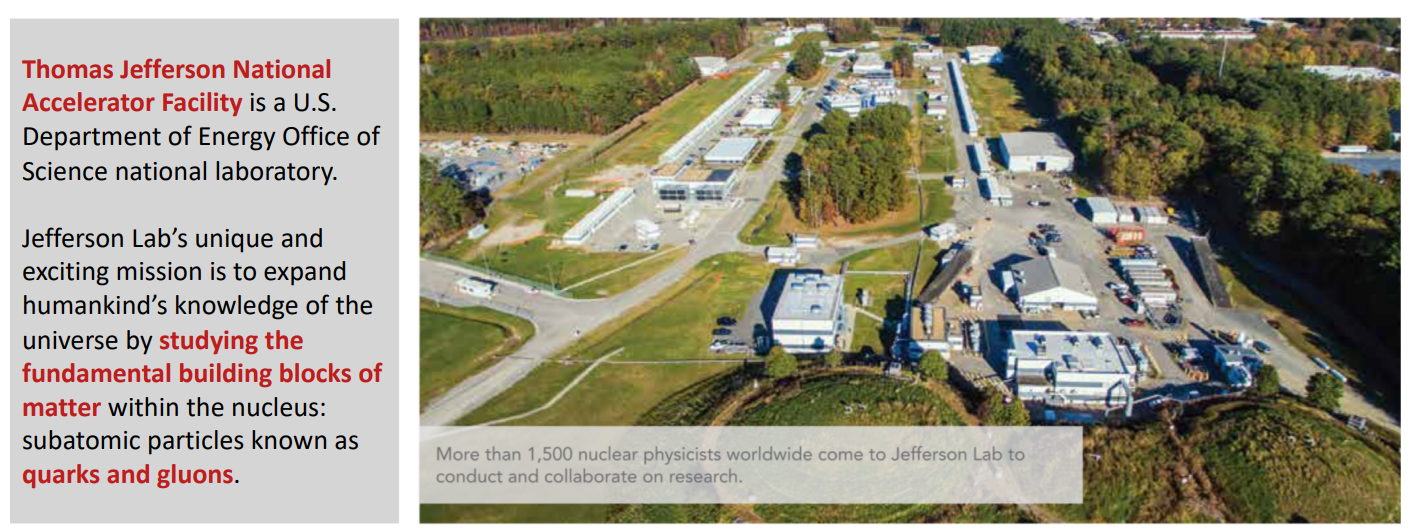
\includegraphics[width=12cm]{../images/Jlab1.png}
\end{figure}
\end{frame}
\begin{frame}{Outline}
\large{
\begin{enumerate}
	\item Deep Inelastic Scattering
	\item The EMC Effect
	\item The MARATHON Experiment
	\item Data Analysis
	\item EMC Effect of A=3
\end{enumerate} 
}

 % Table of contents slide, comment this block out to remove it
	%\tableofcontents % Throughout your presentation, if you choose to use \section{} and \subsection{} commands, these will automatically be printed on this slide as an overview of your presentation
\end{frame}


%----------------------------------------------------------------------------------------
%	PRESENTATION SLIDES
%----------------------------------------------------------------------------------------


\section[DIS]{Deep Inelastic Scattering}


\begin{frame}
%frametitle{DIS Cross Section}
\begin{block}{Deep Inelastic Scattering(DIS) ??????}
\begin{figure}[]
	\centering
	%	\textbf{Electron - Nucleus Scattering   }\par\medskip
	\includegraphics[width=12cm]{../images/Thesis/E_nucleus_spect1.pdf}
	\vspace{20pt}
	\caption*{ Idealized spectra of high-energy electron scattering as a function of energy transfer \cite{spectrum}.}
	
\end{figure}

\end{block}
\end{frame}




\begin{frame}
%frametitle{DIS Cross Section}

\begin{figure}[]
	\centering
	\includegraphics[width=12cm]{../images/Thesis/E_nucleus_spect1.pdf}
\end{figure}

\begin{columns}[t]
	\column{.33\textwidth} % Left column and width
	\only<1>{
	$\bullet$ \textbf{\textcolor{ForestGreen}{Elastic scattering}}
	\begin{figure}[]
		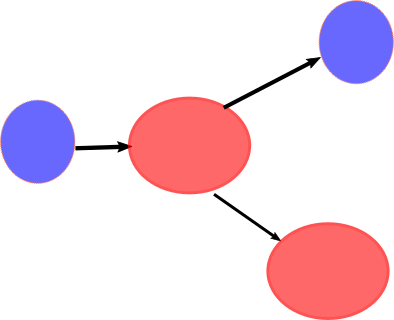
\includegraphics[width=3.5cm,height=3cm]{../images/elast_draw1.png}
	\end{figure}}
	\column{.33\textwidth} % Left column and width
		\only<2>{
	$\bullet$ \textbf{\textcolor{red}{Quaiselastic }}
%	\vspace{-10pt}
	\begin{figure}[]
		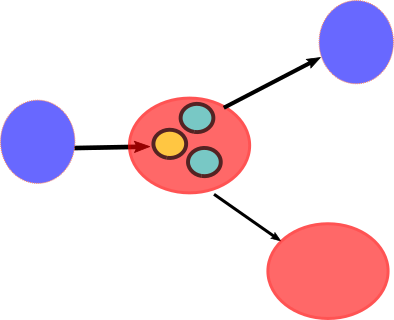
\includegraphics[width=3.5cm,height=3cm]{../images/quais_draw1.png}
	\end{figure}}
	\column{.33\textwidth} % Left column and width
		\only<3>{
	$\bullet$ \textbf{\textcolor{blue}{DIS}}
%	\vspace{8pt}
	\begin{figure}[]
		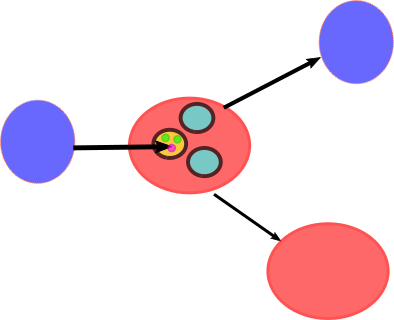
\includegraphics[width=3.5cm,height=3cm]{../images/dis_draw1.png}
	\end{figure}}
	
\end{columns}
\end{frame}


\begin{frame}
\frametitle{Deep Inelastic Scattering (DIS)}
\vspace*{-20pt}
\begin{columns}[c] % The "c" option specifies centered vertical alignment while the "t" option is used for top vertical alignment
	\column{.45\textwidth} % Left column and width
	\begin{figure}
		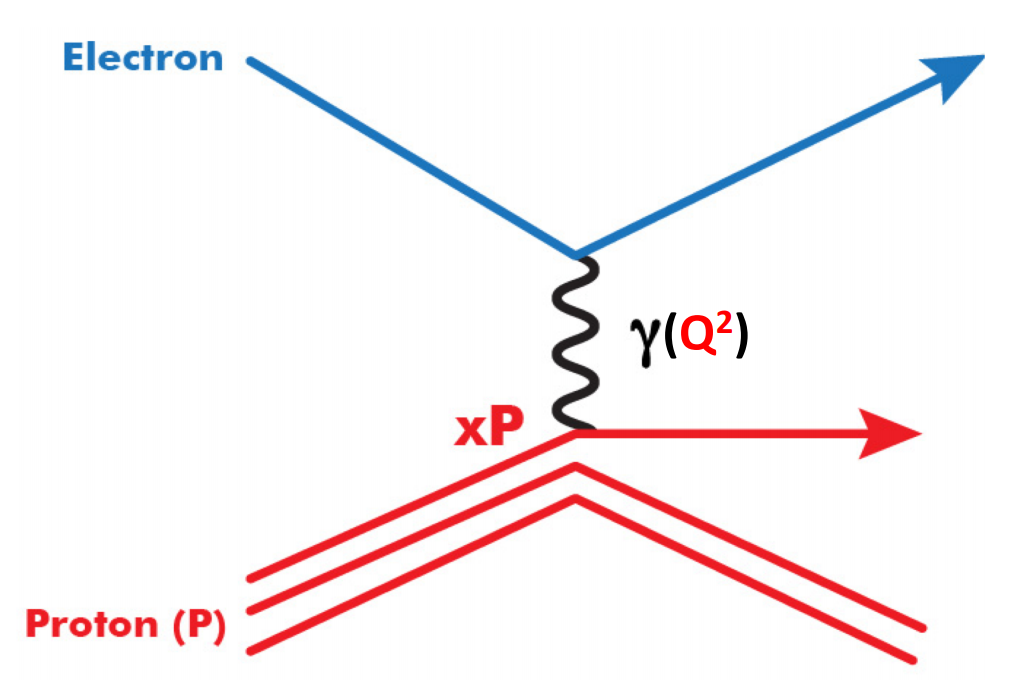
\includegraphics[width =5cm]{../images/DIS_toon.png}
	\end{figure}
	\column{.55\textwidth} % Right column and width
	\pause
	\begin{itemize}
		\item $ Q^2 \equiv 4EE' sin^2 \frac{\theta}{2} $
		\pause
		\item $\nu$ $\equiv$ E-E$^{\prime}$
		\pause
		\item $X_{Bj}= \frac{Q^2}{2\nu M}$
		\pause
		\item  $W^2 = 2M\nu + M^2 - Q^2$
		
	\end{itemize}
\end{columns}
\vspace*{10pt}

\end{frame}

\begin{frame}
\frametitle{Why DIS?}
\vspace*{-15pt}
\centering
\large	$\sigma_{eN} = \frac{\alpha^2}{4E^2sin^4(\frac{\theta}{2})} [\frac{F_2(x)}{\nu}cos^2\left(\frac{\theta}{2}\right) + \frac{2F_1(x)}{M}sin^2\left(\frac{\theta}{2}\right)] $

\begin{columns}[c] % The "c" option specifies centered vertical alignment while the "t" option is used for top vertical alignment
\column{.5\textwidth} % Left column and width	
	\textbf{Quark parton model}\\
	In the Broken limit
\begin{itemize}
	\item $F_2(x) = x \cdot$ $\sum_{i}$ $z_i^2f_i(x) $
	\item $F_1(x) = 1/2 \cdot$ $\sum_{i}$ $z_i^2f_i(x)$
	\item  \textbf{Spin 1/2 quarks} $F_2(x) = F_1(x) \cdot2x$
\end{itemize}



\column{.5\textwidth} % Left column and width
\vspace*{-5pt}
\begin{figure}[t]
	\centering
	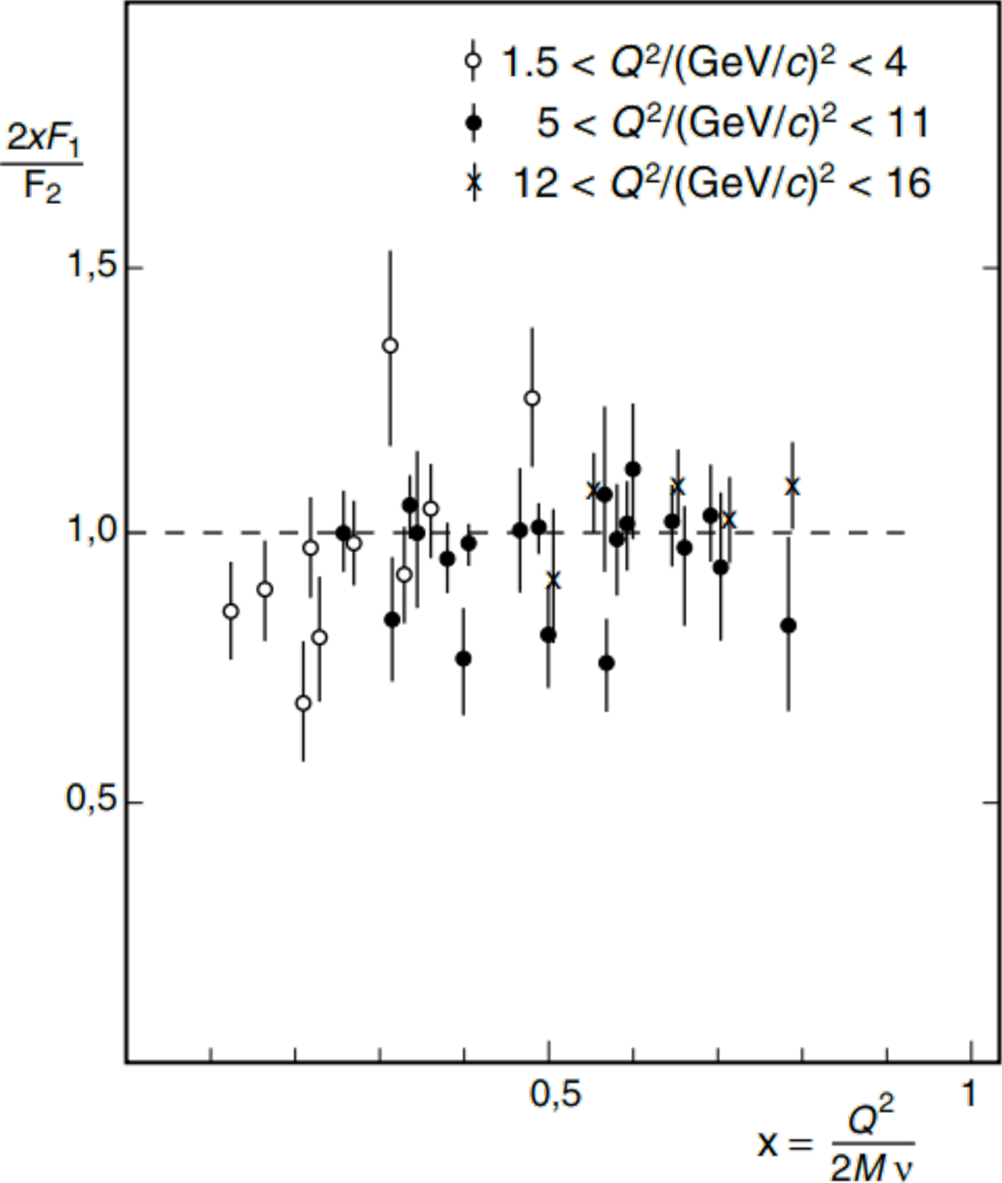
\includegraphics[width=4.5cm]{../images/Thesis/f1_f2_spin.pdf} 
	\caption*{Ratio of $2x\cdot F_1(x)$ and $F_2(x)$ vs. $x$. \cite{PnN}}
	
\end{figure}  
\end{columns}
\end{frame}

%----------------------------------------------------
\section[EMC]{The EMC Effect}

\begin{frame}
\frametitle{The EMC Effect}
\begin{columns}[t]
	\column{.55\textwidth}
	\vspace{-35pt}
	\begin{figure}
		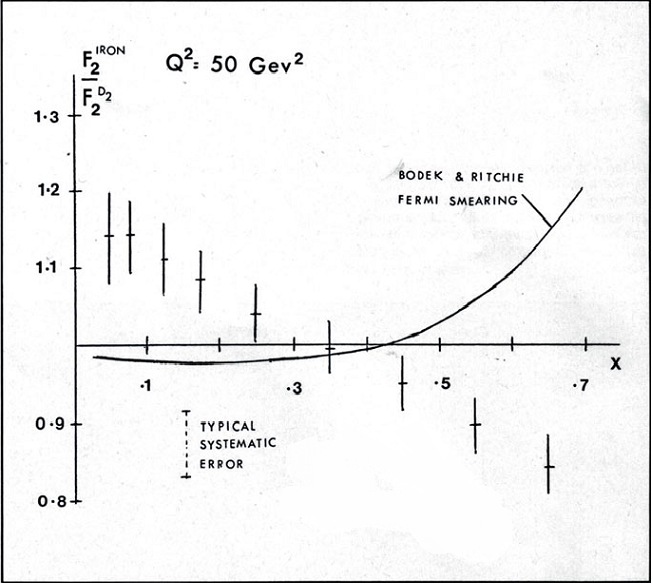
\includegraphics[width =7cm]{../images/Thesis/EMC.png}
		\caption*{\cite{cc}}
	\end{figure}
	\column{.45\textwidth}
	
	\vspace{-1.25cm}	\hspace{-20pt}\textbf{ European Muon Collaboration}
	
	\begin{itemize}
		\item \small$X$ = fraction of momentum carried by quark	
				\pause
		\item Expected Unity at low $x$ 
				\pause
		\begin{itemize}
			\item Binding $<$ momentum transfer
			\item Free Nucleons
		\end{itemize}

		\item F$^A$ = $Z \cdot F^p + (A-Z)\cdot F^n$  
		\pause
		\item Unexpected Relative Decrease
		\item Missing high-momentum quarks in A$>$2
		\pause
		\item EMC Effect $\equiv$ structure of the A/D Ratio
	\end{itemize}
	
\end{columns}
\end{frame}
%----------------------------------------------



\begin{frame}{The EMC Effect}

\begin{figure}
\caption*{\label{EMC_slac} SLAC experiment E139 \cite{slac_emc} .}
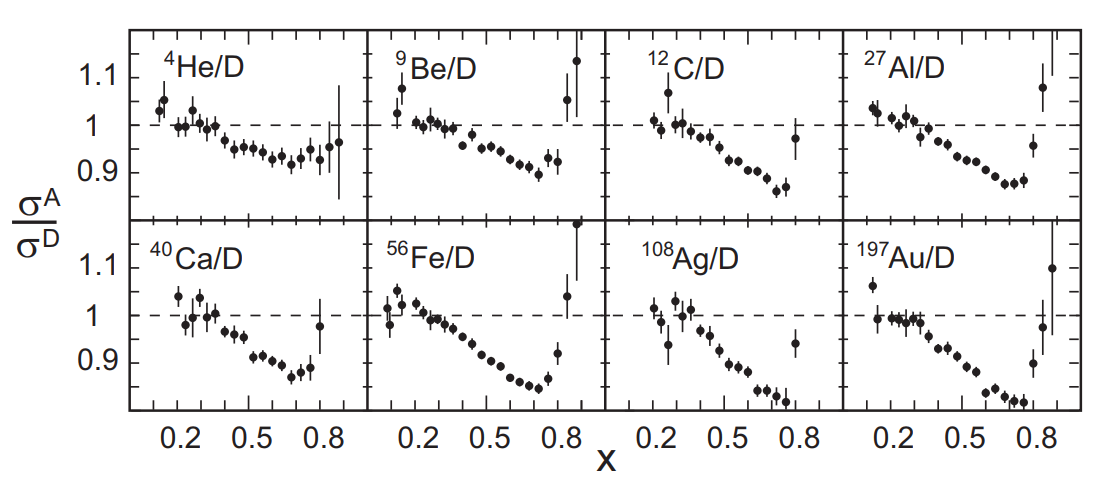
\includegraphics[width =12cm]{../images/EMC_slac_horiz.png}
\end{figure}


\end{frame}

%----------------------------------------------
\begin{frame}
\begin{columns}
\column{.5\textwidth} % Left column and width
\vspace{-20pt}
\begin{figure}
	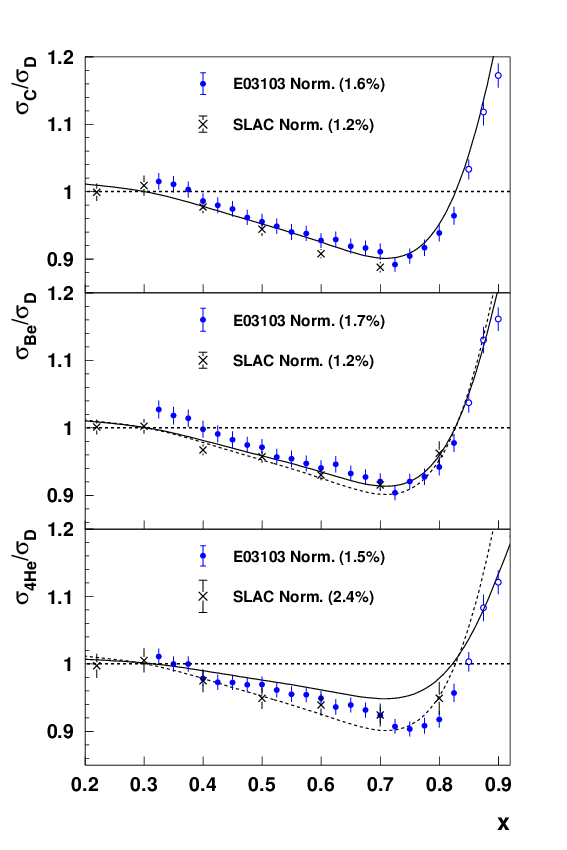
\includegraphics[width=6cm]{../images/carbon_be_he4}
\end{figure}
\column{.50\textwidth} % Left column and width

{\hspace*{50pt}
	\begin{itemize}
		\item<1-> JLab experiment E03103 \cite{E3103} 
		\item<2-> CERN, SLAC, HERMES, BCDMS, and JLab
		\item<3-> Quantized by slope of A/D ratios from 0.3 - 0.7 in x
		\item<4-> Models have difficulty matching data for all criteria
		\item<5-> $\approx$ log dependence in A
	\end{itemize}
}
\end{columns}
\end{frame}

\begin{frame}{The EMC Effect}
\begin{columns}
	\column{.65\textwidth} % Left column and width
	\vspace{-35pt}
	\begin{figure}
		\caption*{JLab experiment E03103 \cite{E3103} }
%		\vspace{10pt}
		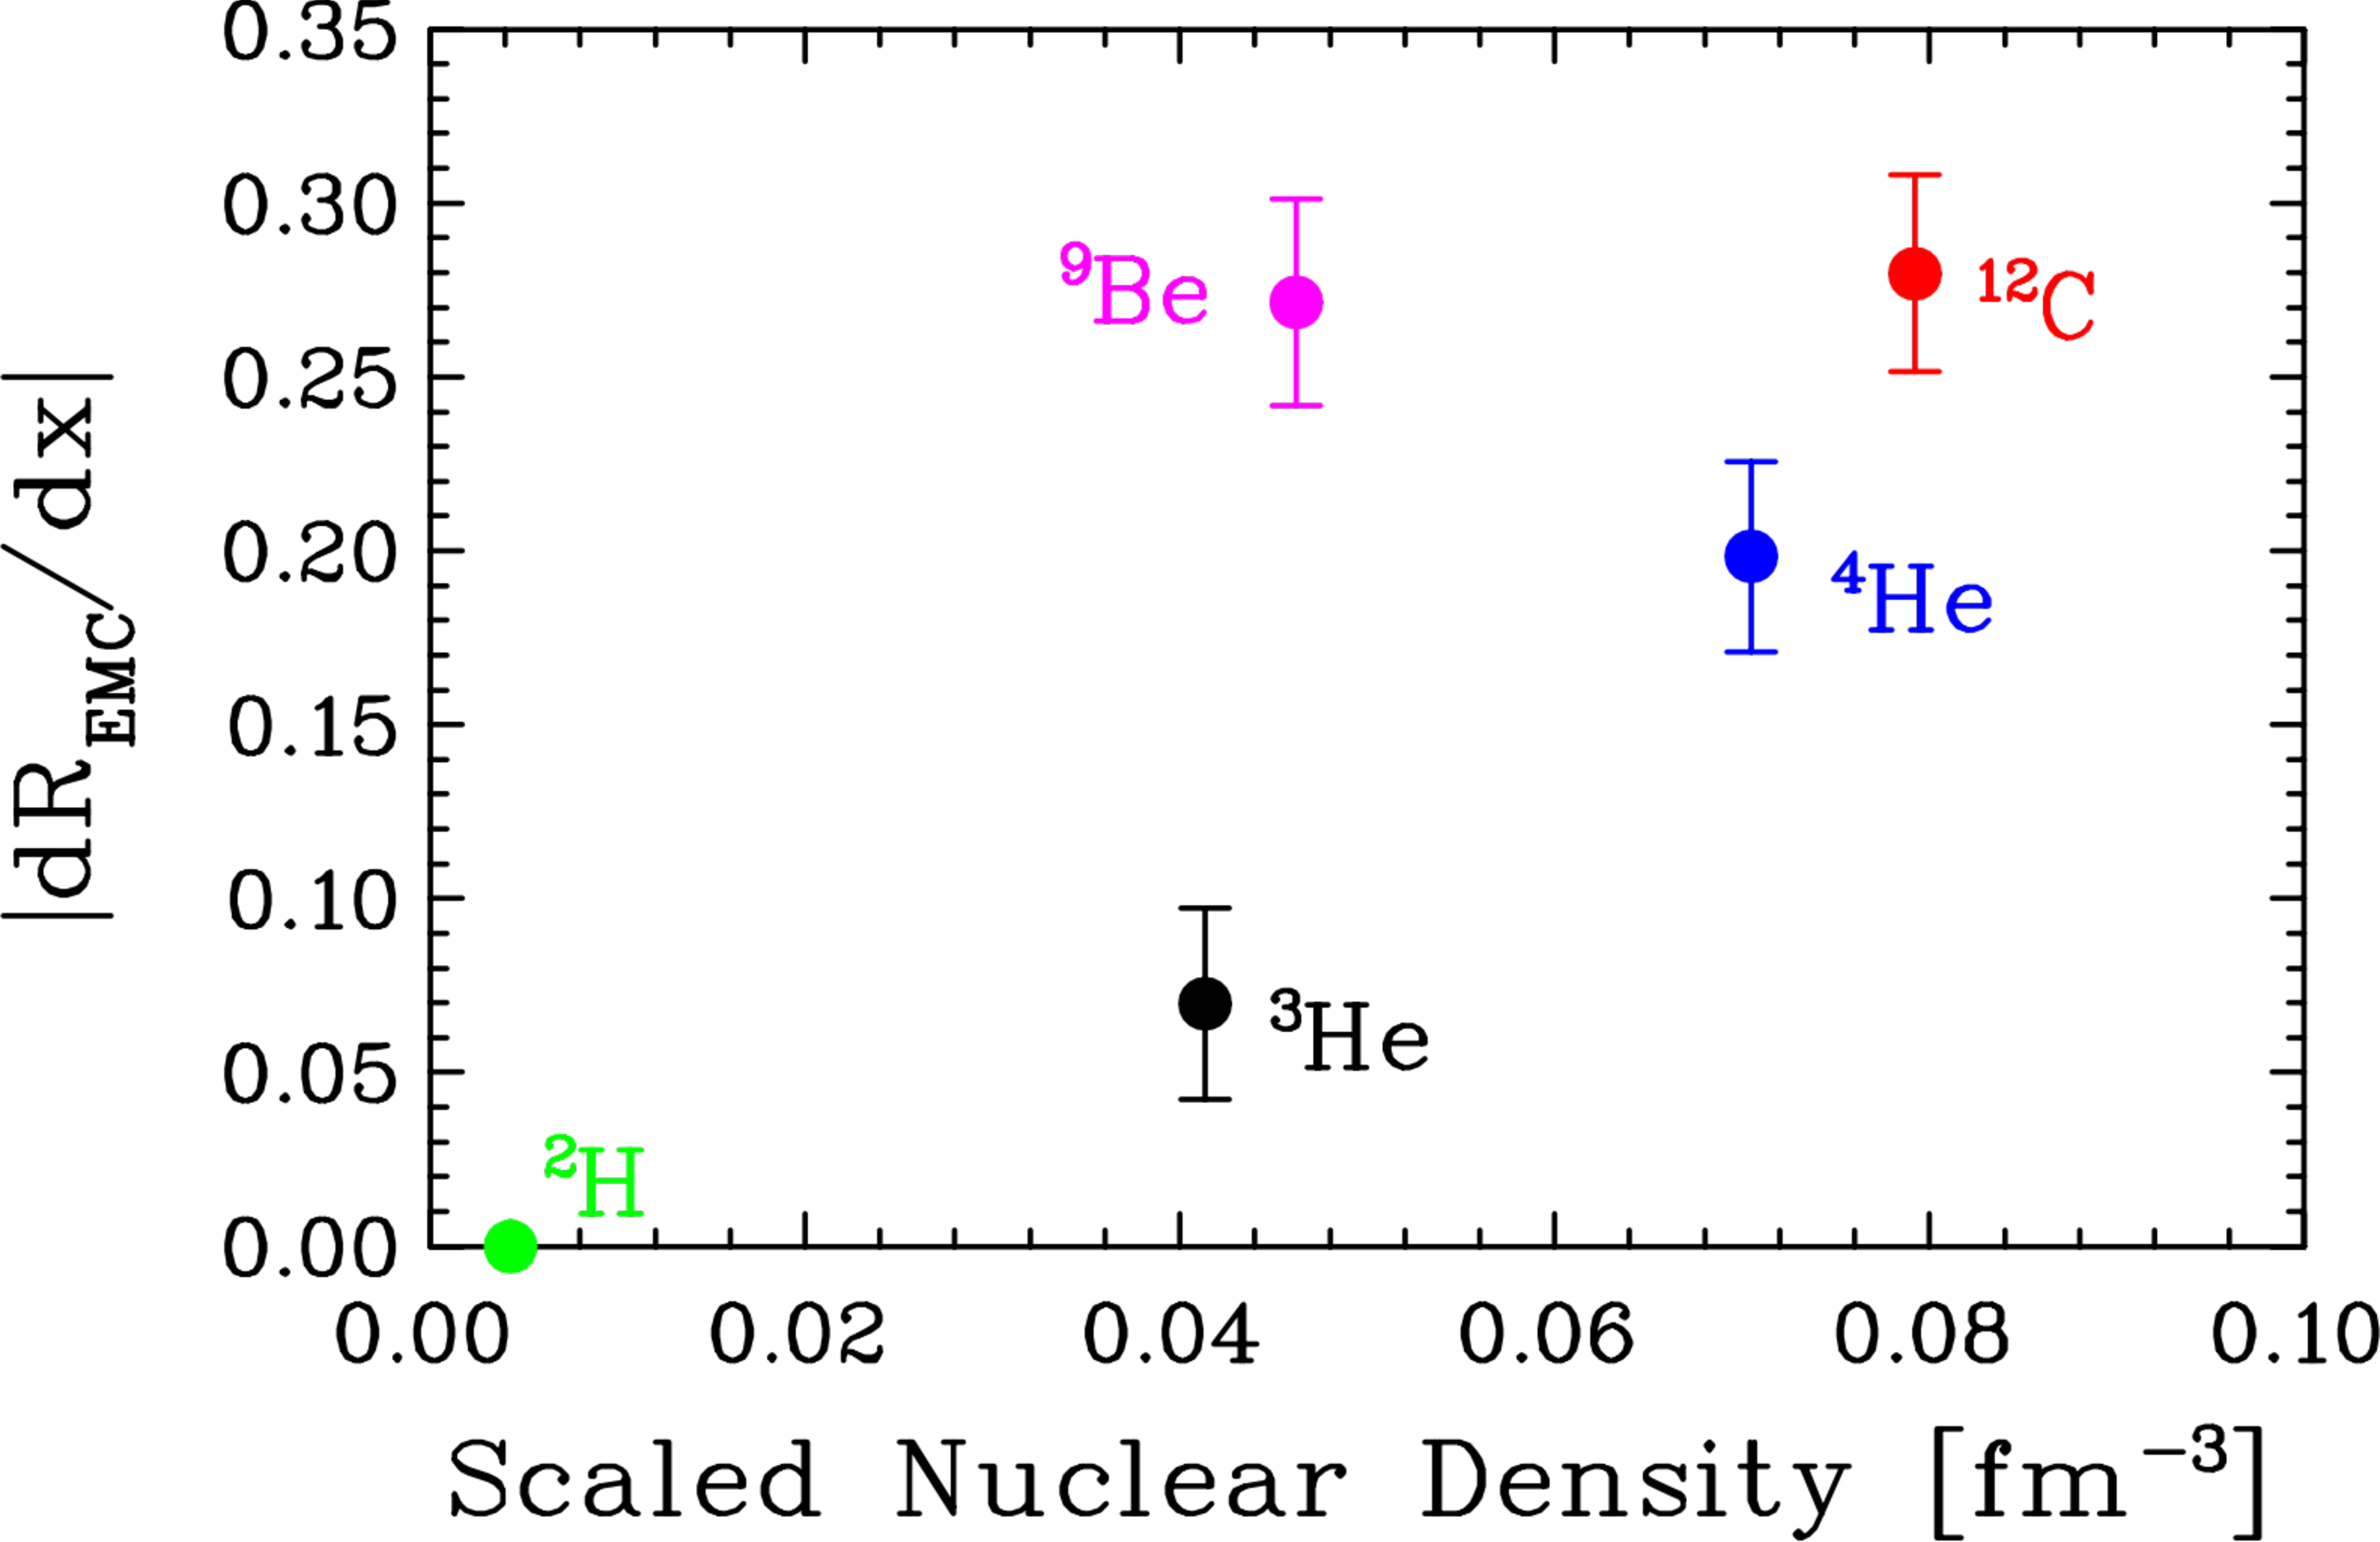
\includegraphics[width =8cm]{../images/Thesis/EMC_rho.pdf}
	\end{figure}
\pause
	\column{.33\textwidth} % Left column and width

	{\centering
	{\vspace{-20pt}	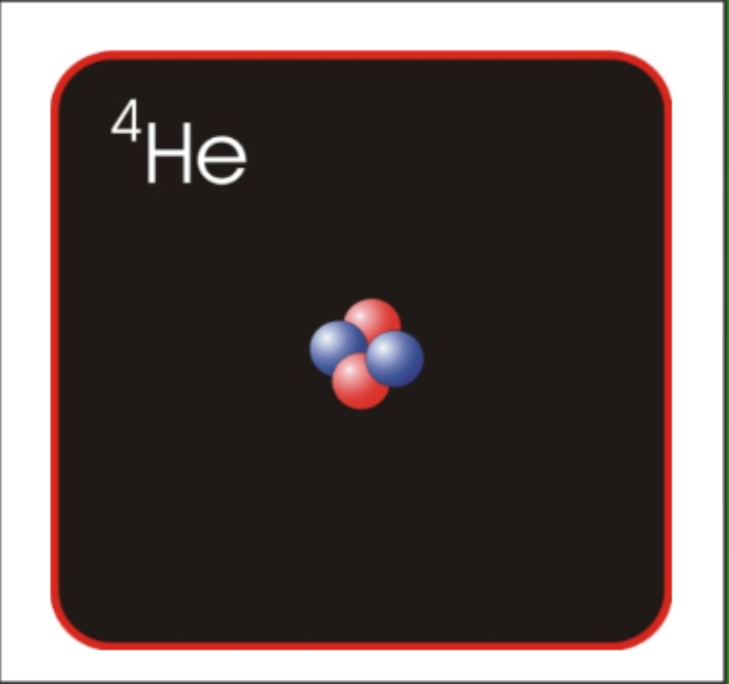
\includegraphics[width=4.cm]{../images/He4.png}}
	{\vspace{5pt}	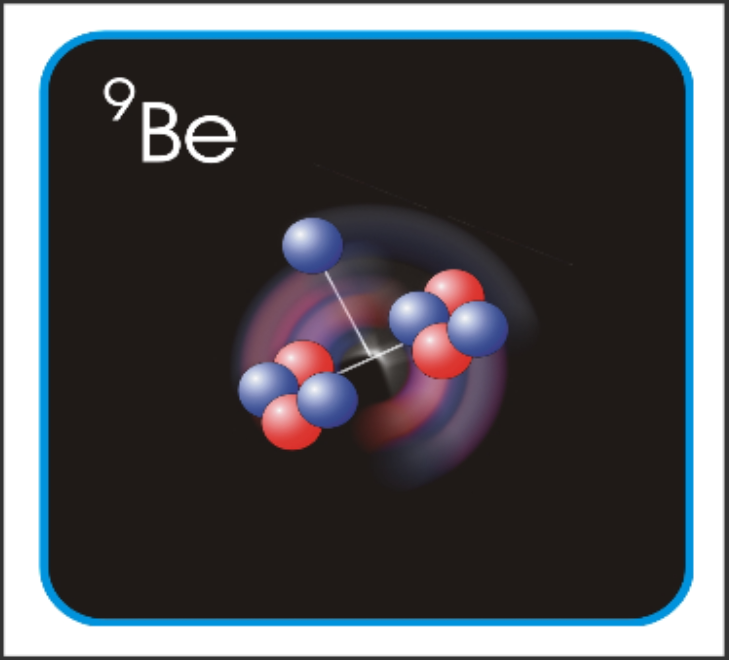
\includegraphics[width=4.cm]{../images/Be9.png}}
	}
%	\hspace{10pt}

\end{columns}
\end{frame}

\begin{frame}{EMC Models}
\vspace{-0.5cm}
\begin{block}{Multiquark Cluster}
	\begin{itemize}
		\item Possible formation of color singlet quark clusters
		\item Clusters contain momentum of multiple nucleons
		\item Multiquark bag should be large compared to nucleon
		\begin{itemize}
			\item softer momenta
			\item Could explain rapid rise in EMC ratio
		\end{itemize}
	\end{itemize}
\end{block}
\only<1>{
	\centering
	\begin{figure}
		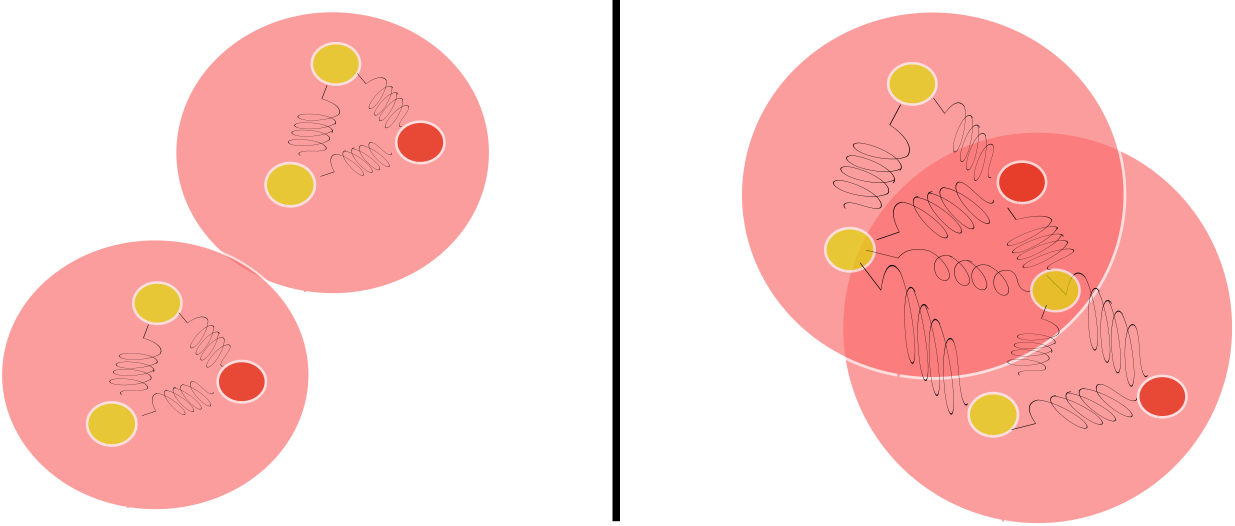
\includegraphics[width=8cm]{../images/bagmodel.png}
	\end{figure}}
\pause
\begin{block}{Nuclear Binding}
	\begin{itemize}
		\item Convolution of momentum and separation energy $\vec{p^{\prime}} = (M + \epsilon, \vec{p})$
		\item Smearing in $x$ 
		\item Can explain the EMC effect region 
		\item Fails to reproduce the rising around $x$ of 0.2
	\end{itemize}
\end{block}
\end{frame}
\begin{frame}{EMC Models}
\vspace{-0.5cm}
	\begin{block}{Medium Modification}
		\begin{itemize}
			\item Modification of nuclear structure
			\item Fields created by surrounding nucleons
			\item Modification of quark waveform
			\item Shown to describe EMC effect well for a collection of nuclear targets.
		\end{itemize}
	\end{block}
\pause	
	\begin{block}{Rescaling}
		\begin{itemize}
			\item Relate DIS structure functions with scaling variable
			\item $F_2^{Fe}(Q^2) =F_2^{D}(\xi Q^2)$
			\item Large nuclei bound in large area compared to free nucleon
			\item Applicable $\rightarrow$ 0.3 $<$ $x$ $<$ 0.8 
		\end{itemize}
	\end{block}


\end{frame}


\begin{frame}{EMC Models}
\centering Brief summary of a small subset of models.\\
\centering Sources for this discussion and others
\vspace{1cm}
	\begin{itemize}
		\item \cite{EMC_medium_1}
		\item \cite{EMC_model_1}
		\item \cite{Geesaman} 
		\item \cite{Norton} 
		\item \cite{EMC_medium_2} 
	\end{itemize}
\end{frame}


\begin{frame}{The EMC Effect}
\begin{columns}[t]
	\column{.5\textwidth} % Left column and width
	\vspace{-20pt}
	\begin{figure}
		\vspace{-25pt}
		
\includegraphics[width =6cm]{../images/puzzels.jpg}
	\end{figure}
	\column{.55\textwidth} % Left column and width
	\hspace{10pt}
	\begin{itemize}
		\item[]\textbf{The EMC puzzle}
		\item 3+ decades of study
		\item \leavevmode\Ccancel[red]{Every Model is Cool(EMC)} 
		\item Dependence on A
		\item Driven by local density
	\end{itemize}
\end{columns}
\centering The EMC results show a modification to nuclear structure. \\
\centering Are we treating it correctly?
\end{frame}



\section[MARATHON]{MARATHON Introduction}
\subsection[Introduction]{Introduction}
%----------------------------------------------
\iffalse
\begin{frame}
\frametitle{Tritium Experiments}
\vspace*{-25pt}
\begin{figure}
	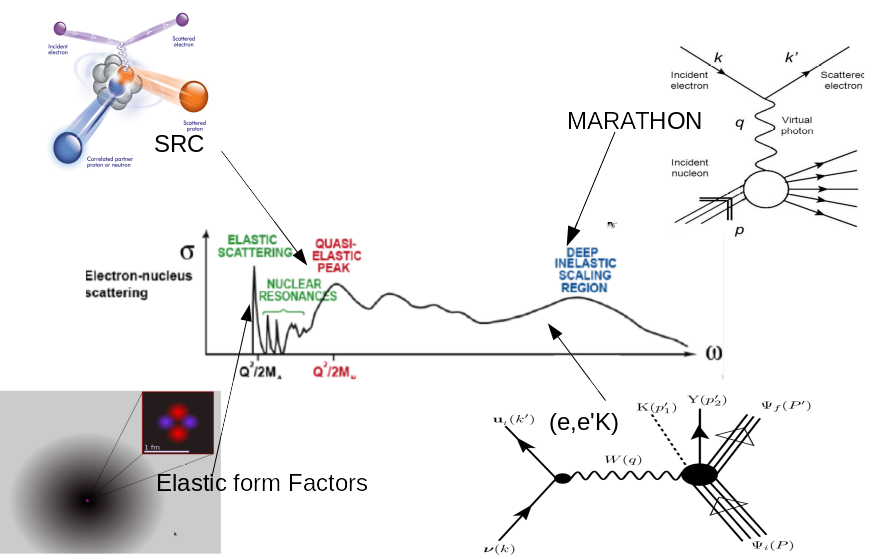
\includegraphics[width =12cm]{../images/tritium_ov}
\end{figure}
\end{frame}
\fi
%----------------------------------------------
\begin{frame}
\frametitle{MARATHON}
\vspace{-10pt}
\begin{block}{}
MeAsurement of $F^n_2/F^p_2, d/u$ RAtios and $A=3$ EMC Effect in Deep Inelastic Electron Scattering off the Tritium and Helium MirrOr Nuclei.
\vspace{-10pt}
\begin{columns}[t]
	
	\column{.35\textwidth} % L column and width
	\vspace{-10pt}	
	\hspace{-10pt}
	\begin{figure}
		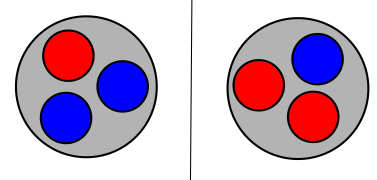
\includegraphics[width =5cm]{../images/mirror}
	\end{figure}
	
	\column{.65\textwidth} % Right column and width
	\vspace{10pt}
	\begin{itemize}
		\item Lightest and simplest mirror system
		\begin{itemize}
			\item  Number of protons in $^3H =$ neutrons in $^3He$
		\end{itemize}
		\item Differences in the nuclear effects are small
		%	\item Improve the current measurement and understanding of $F^n_2/F^p_2$ ratio
		%	\item Restrict the assumptions and parameters made in the model calculations of the down to up quark distribution ratio
	\end{itemize}
	
	
\end{columns}
\end{block}
\end{frame}
\begin{frame}
\frametitle{The JLab MARATHON Tritium Collaboration}
\vspace{-15pt}

\begin{figure}
	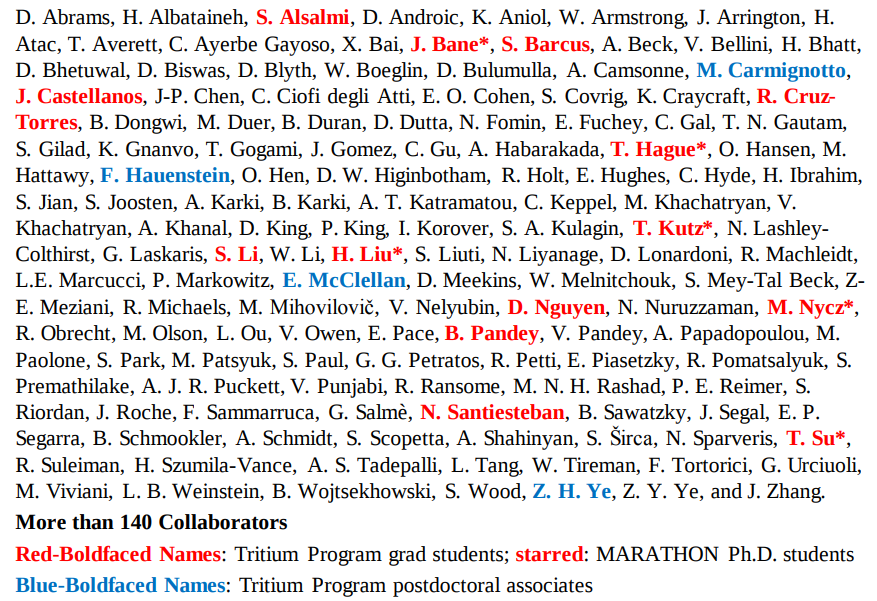
\includegraphics[width =11.5cm]{../images/collabos_ppl.png}
\end{figure}

\end{frame}

\begin{frame}
\frametitle{The JLab MARATHON Tritium Collaboration}
\vspace{-15pt}

\begin{figure}
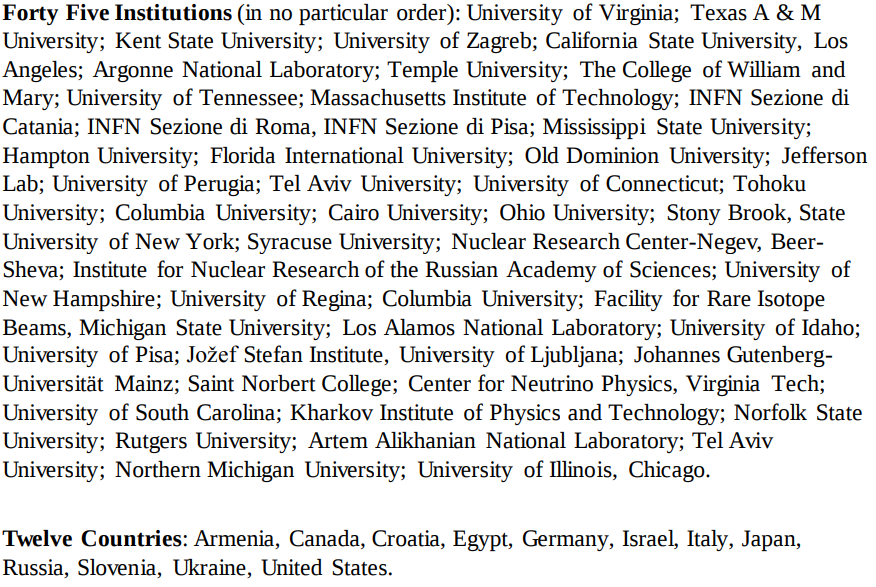
\includegraphics[width =11.5cm]{../images/callabos_un.png}
\end{figure}

\end{frame}
%----------------------------------------------
%----------------------------------------------
\section[Experiment]{The Experimental Setup}
\subsection[Equipment]{The Experimental Setup}

\begin{frame}
The Continuous Electron Beam Accelerator Facility (CEBAF) at Thomas Jefferson Accelerator Facility.\\

\vspace{-10pt}
\begin{columns}[c]
	\column{.52\textwidth}
		\begin{figure}
			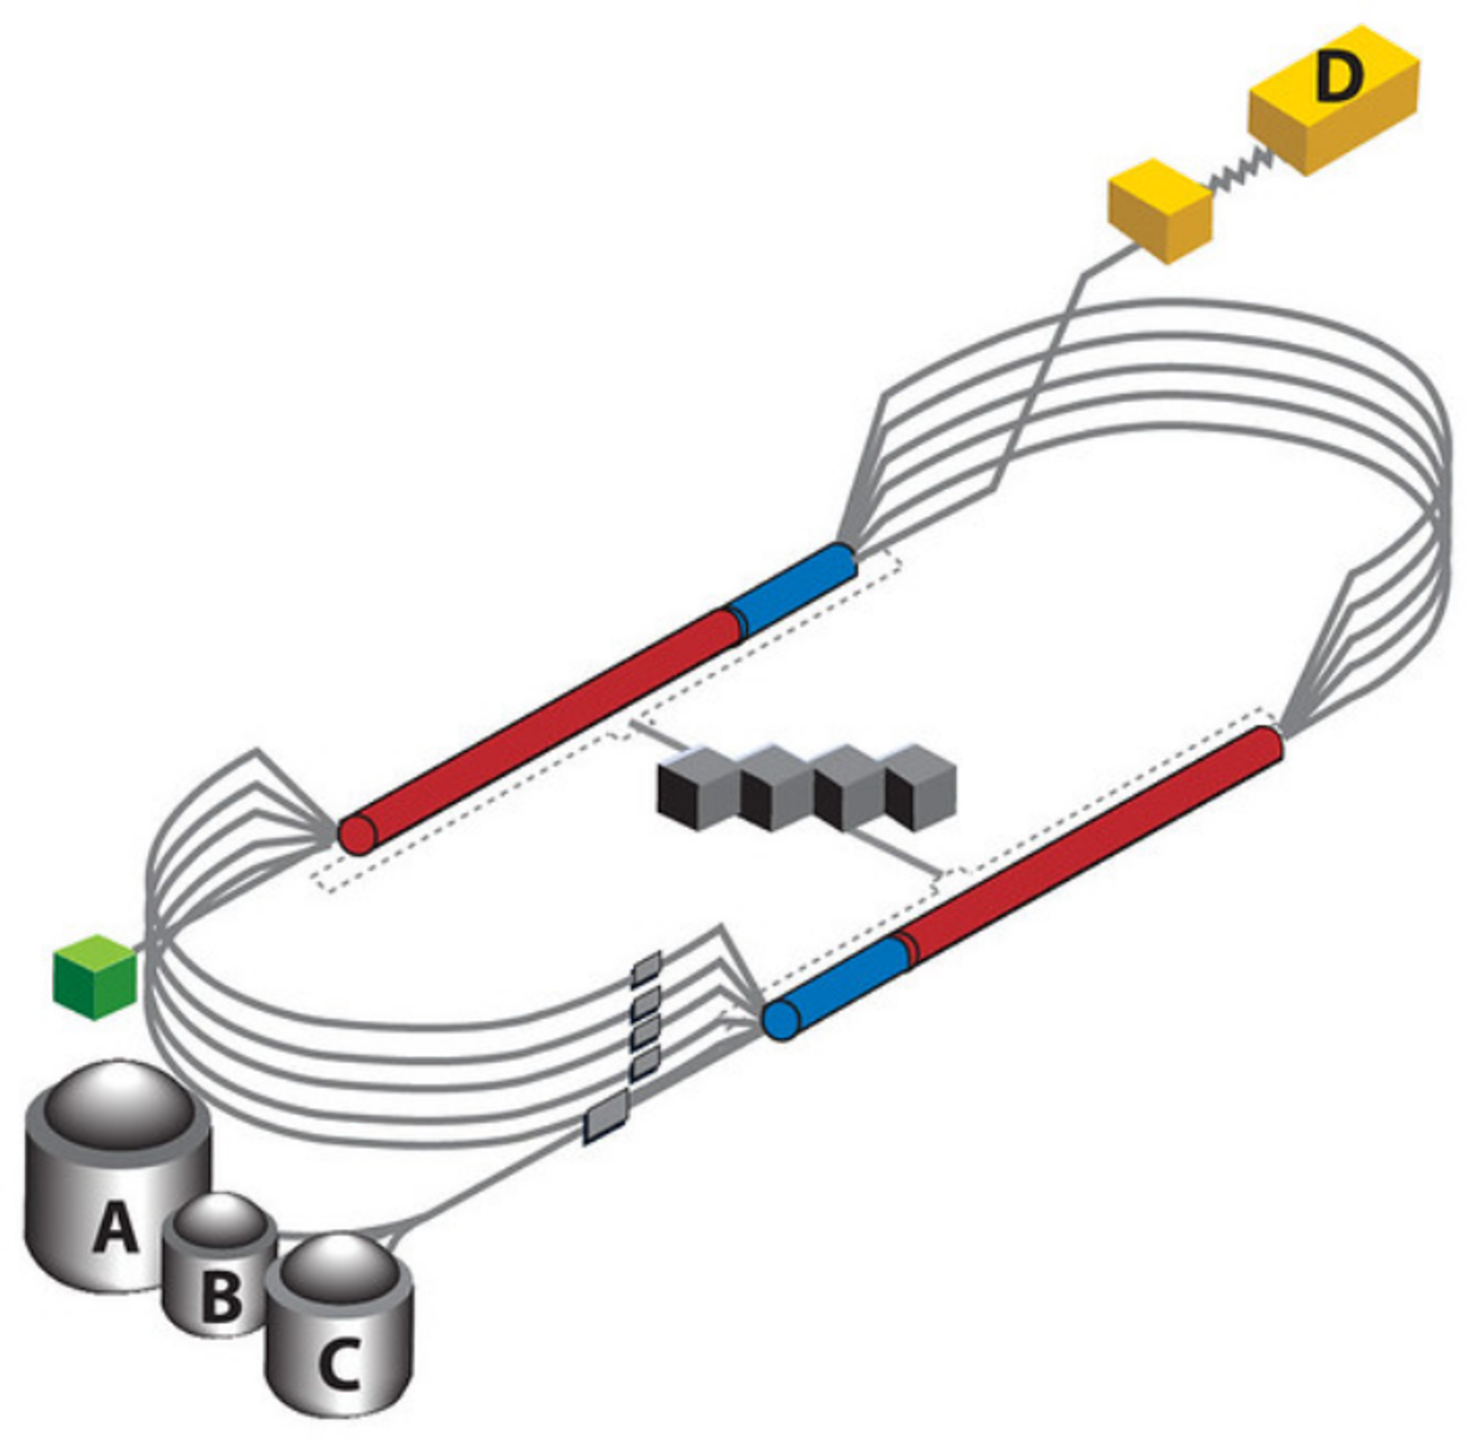
\includegraphics[width=5.5cm]{../images/cebaf.pdf}
		\end{figure}
	\column{0.48\textwidth}
		\begin{block}{}
			\begin{itemize}
				\addtolength{\itemindent}{-1em}
				\item $\approx$ 2.2 GeV per revolution
				\item 12 GeV for Hall D
				\item Superconducting RF cavities
				\item RF separators split the beam to each Hall
				\item [] \hspace{-15pt}\textbf{MARATHON's proposal }
				\item 11 GeV Beam	
			%	\item Bigbite spectrometer
				\item Hall A's high resolution spectrometers (HRS)
				\item Tritium
			\end{itemize}
		\end{block}
\end{columns}
\end{frame}


\begin{frame}
\begin{center}
	\textbf{Uses of Tritium}
	\begin{tikzpicture}
	\node (img1) {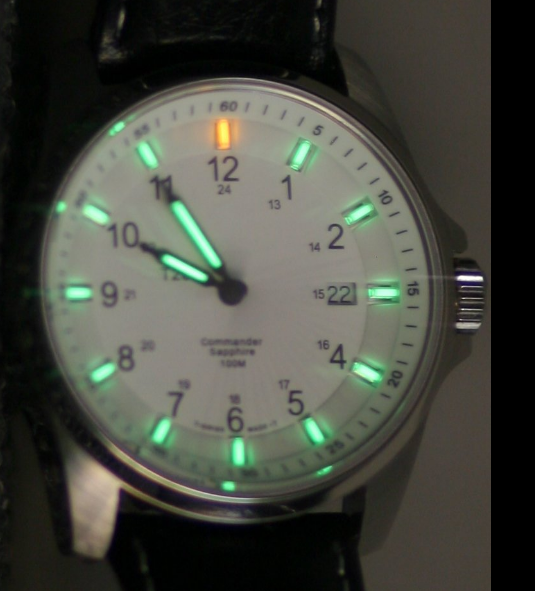
\includegraphics[height=5cm]{../images/T1.png}};
	
	\node (img2) at (img1.south east)[xshift=2.5cm,yshift=3cm] {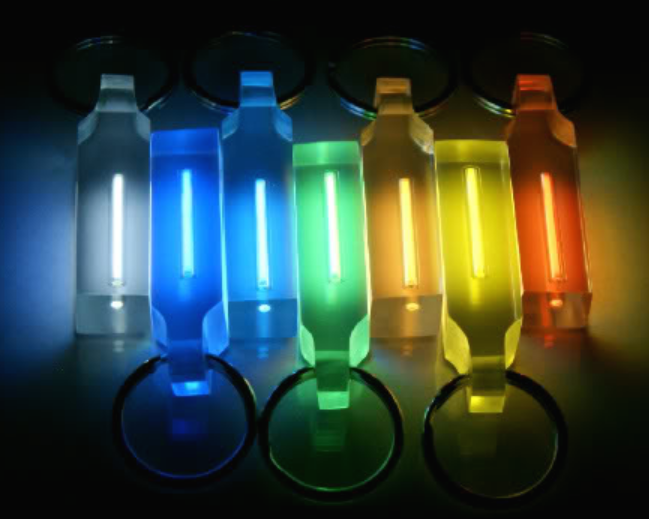
\includegraphics[height=4cm]{../images/T2.png}};
	
	\node (img3) at (img2.south west) [yshift=-1.5cm] {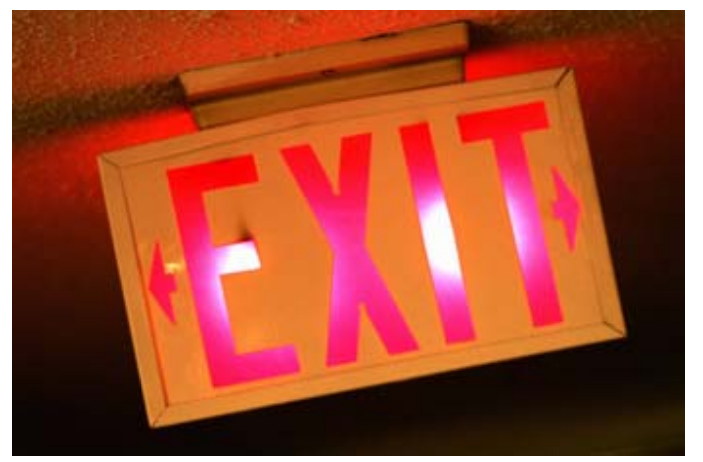
\includegraphics[height=4cm]{../images/T3.png}};
	\end{tikzpicture}
\end{center}
\end{frame}


%---------------------------------------------------------------
\begin{frame}
\frametitle{Tritium Target Cell}
\begin{columns}[]
	\column{0.45\textwidth}
	First tritium target at JLab
	\begin{itemize}
		\item Thin Al entrance and exit windows ~0.01 inches
		\item 1090Ci of Tritium (0.1 g)
		\item 25 cm long
		\item Tritium Cell was filled in Savannah River
		\item 40 kelvin Helium is used to cool an attached heat sink
	\end{itemize}
	\column{0.45\textwidth}
	\begin{figure}
		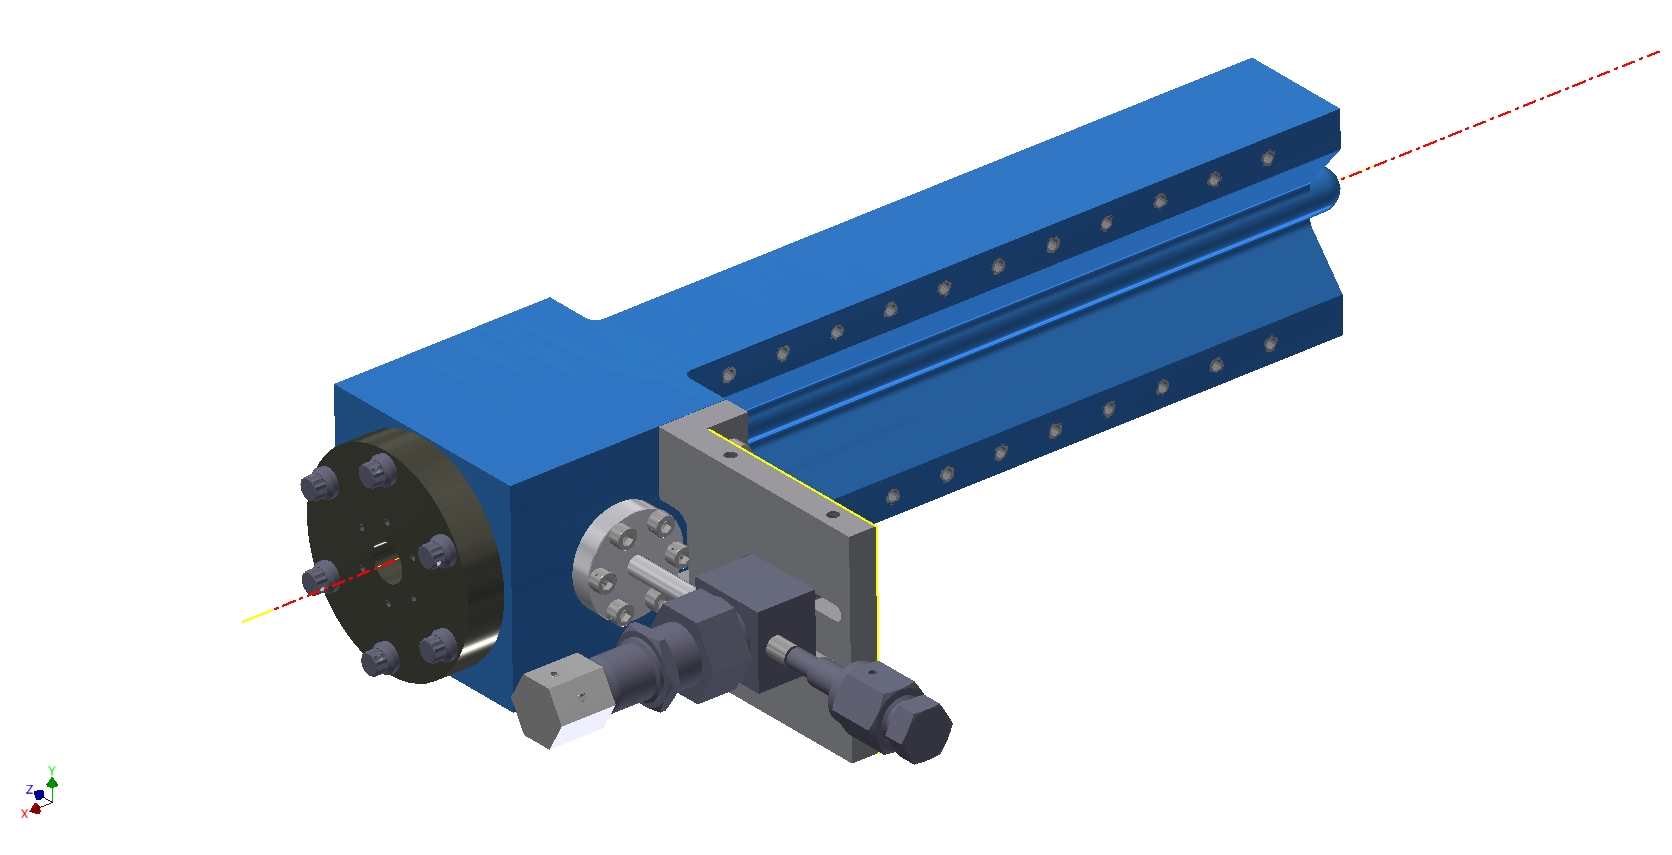
\includegraphics[width=5cm]{../images/tgt_cell}
	\end{figure}
	\vspace{-10pt}
	\begin{figure}
		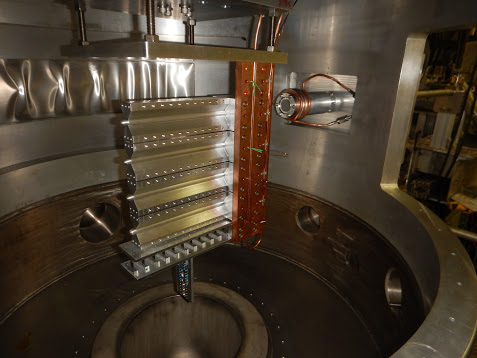
\includegraphics[width=5cm]{../images/tag_lat}
	\end{figure}
\end{columns}
\end{frame}

%----------------------------------------------

\begin{frame}
\frametitle{Hall A}
\begin{figure}
	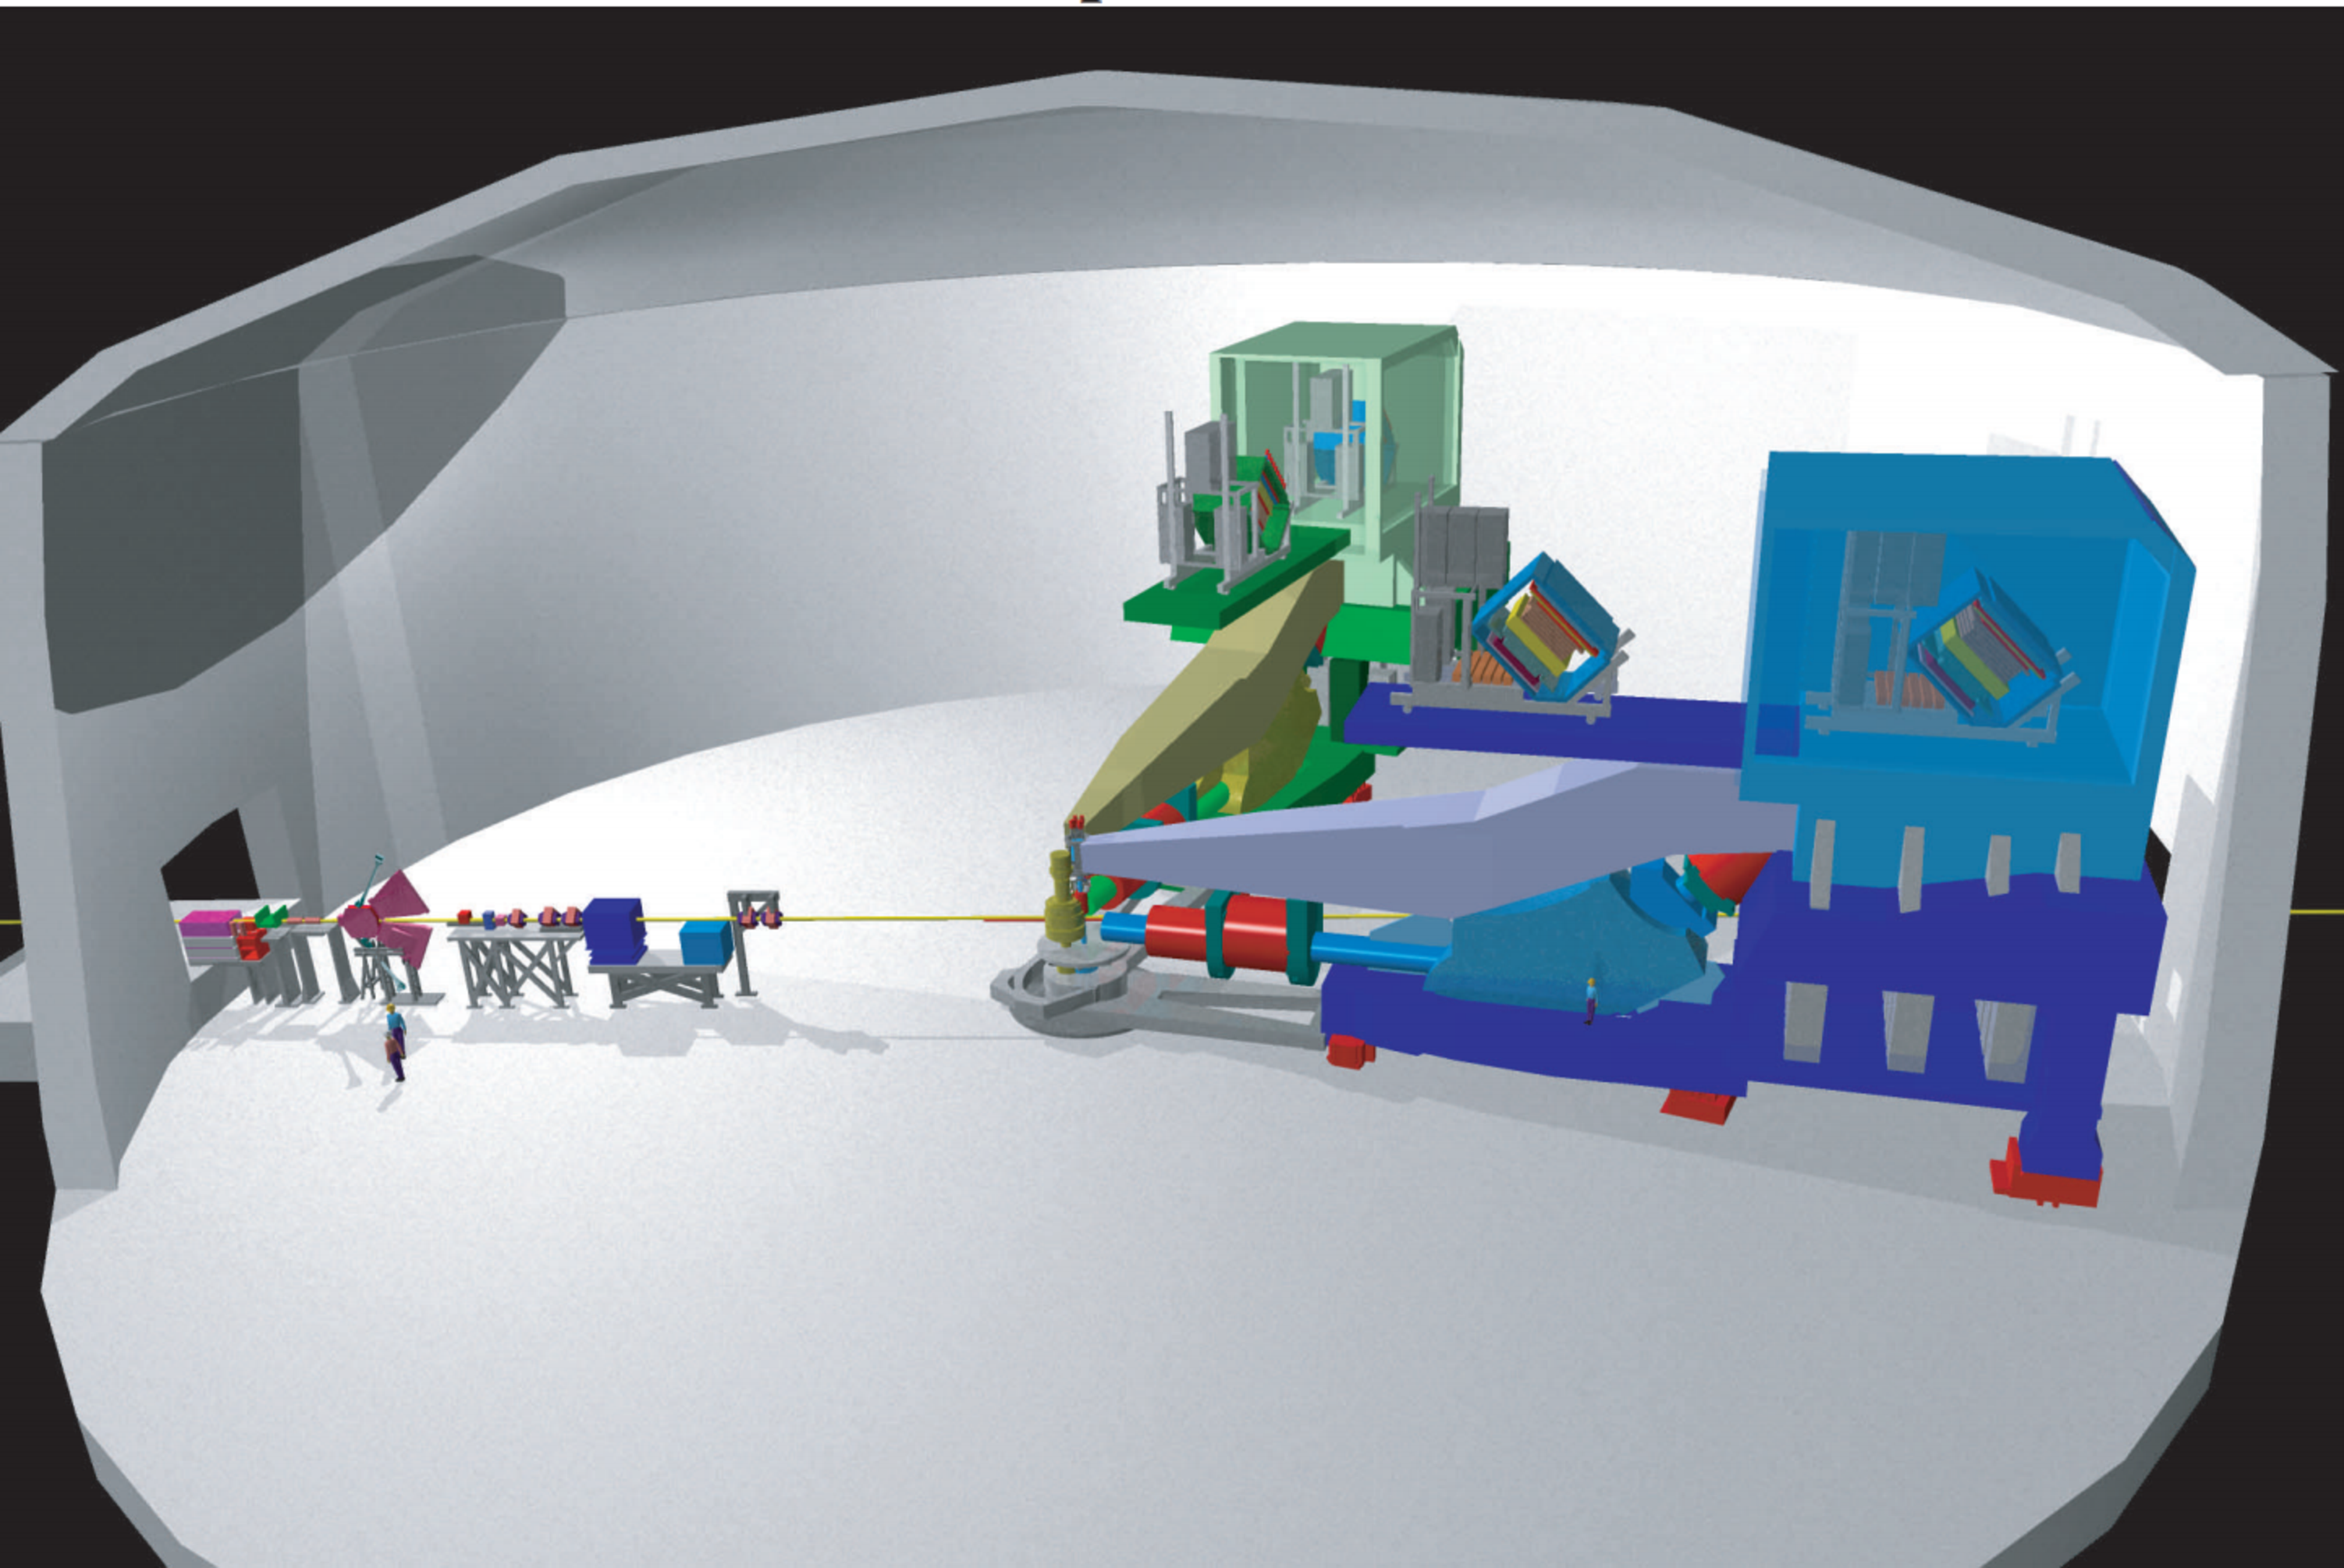
\includegraphics[width=10.5cm]{../images/halla.pdf}
\end{figure}
\end{frame}

%---------------------------------------------------------------
\begin{frame}
\frametitle{High Resolution Spectrometers (HRSs)}
	\begin{figure}
		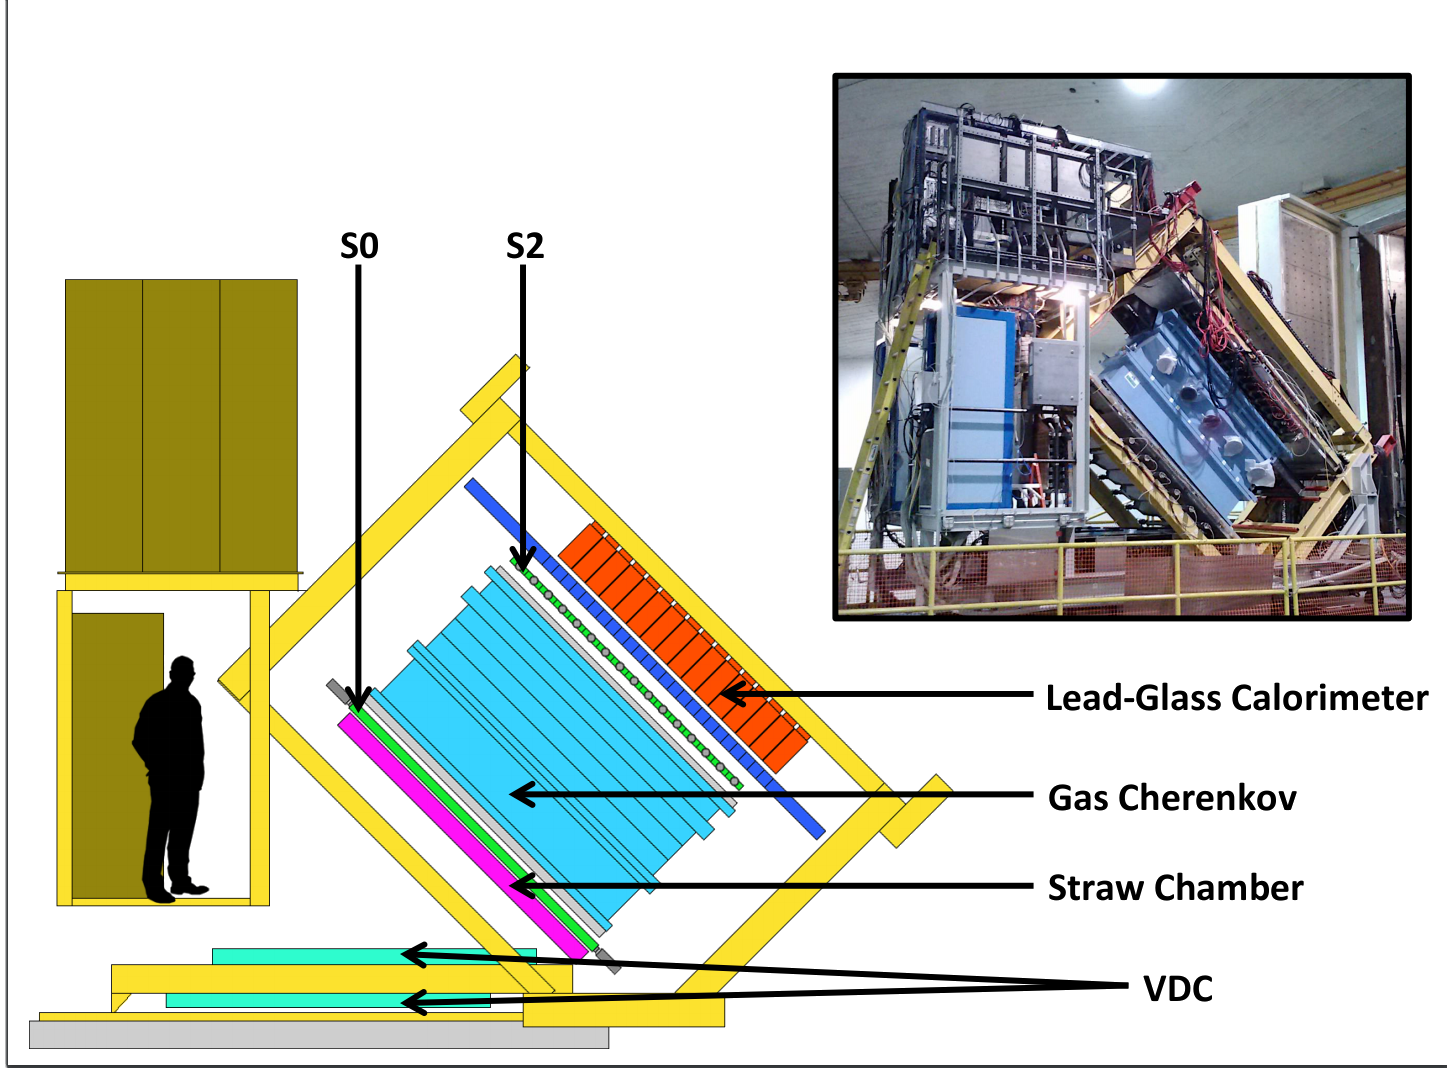
\includegraphics[width=10cm]{../images/HRS_cartoon}
	\end{figure}
\end{frame}





%-----------------------------------------------
\iffalse
\begin{frame}
\centering 
\textbf{Bigbite Spectrometer}
\begin{columns}
	
	\column{0.5\textwidth}
	\begin{figure}
		\hspace*{-1.4cm}	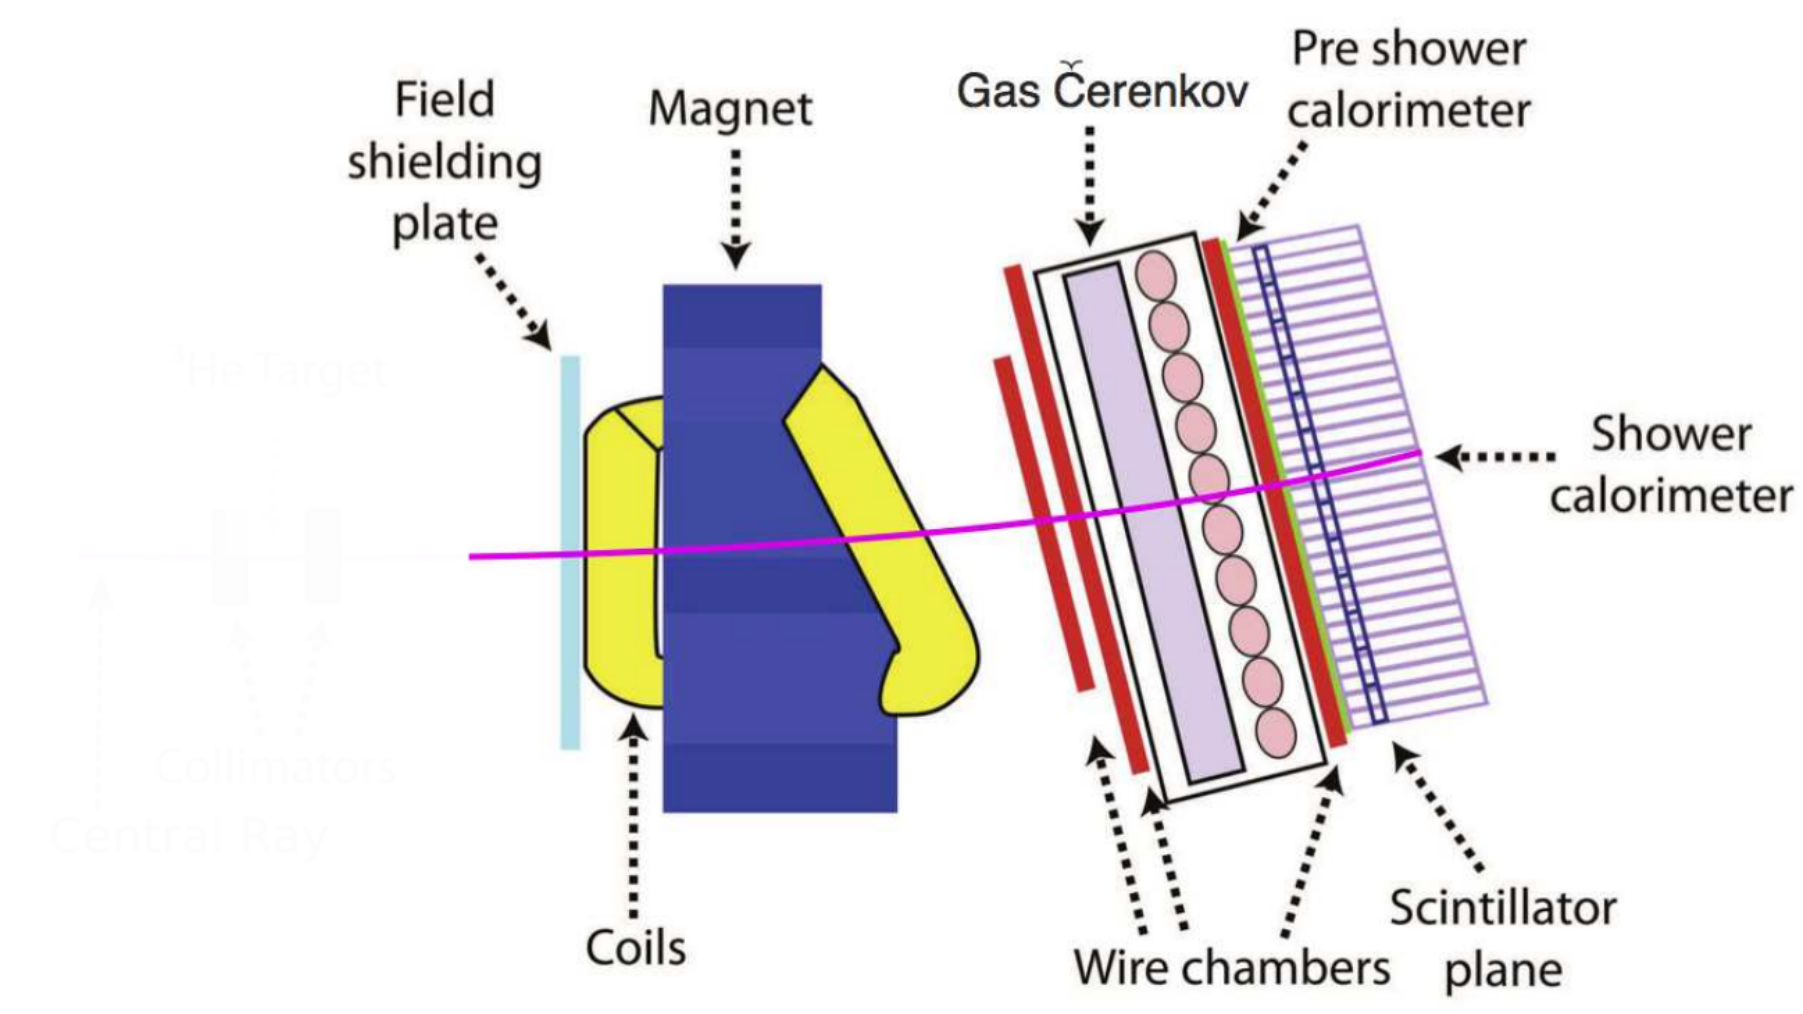
\includegraphics[width=7cm]{../images/Thesis/BigBite1.png}
	\end{figure}
	\begin{block}{}
		\begin{itemize}
			\item[] \noindent Large Acceptance Spectrometer
			\item Solid angle = 96 mrad
			\item Large Momentum Acceptance: $>$ 500 MeV/c
		\end{itemize}
	\end{block}
	
	\hspace*{0.5cm}
	\column{0.5\textwidth}
	\begin{block}{My contributions in preparing Bigbite}
		\begin{itemize}
			\item Constructing the data acquisition system
			\item PMT performance studies
			\item Designing trigger logic
			\item Ensuring consistent and dependable HV power
		\end{itemize}
		Removed from the run plan for safety and logistical concerns
	\end{block}
\end{columns}
\end{frame}
\fi
%----------------------------------------------



\subsection[Run Period]{Run Period}
\begin{frame}
\frametitle{The Run Period}
\vspace{-20pt}
\begin{columns}
	\column{0.35\textwidth}	
	\begin{figure}
		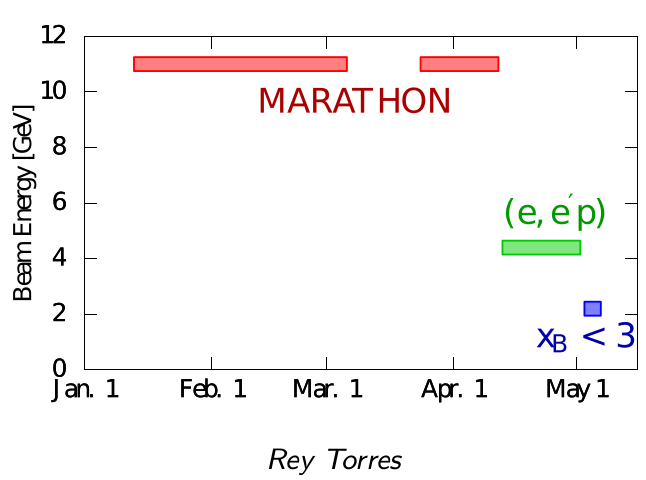
\includegraphics[width=4.5cm]{../images/run_per}
	\end{figure}
	\column{0.65\textwidth}
	\vspace{-10pt}
	\begin{itemize}
		\item Ran from January 11th to April 12th of 2018.
		\item Gaseous targets - Tritium, Deuterium, Helium-3, and Hydrogen
		\item Rotated through targets to achieve equal statistics and reduce the impact of systematic uncertainties
	\end{itemize}
\end{columns}
\begin{figure}
	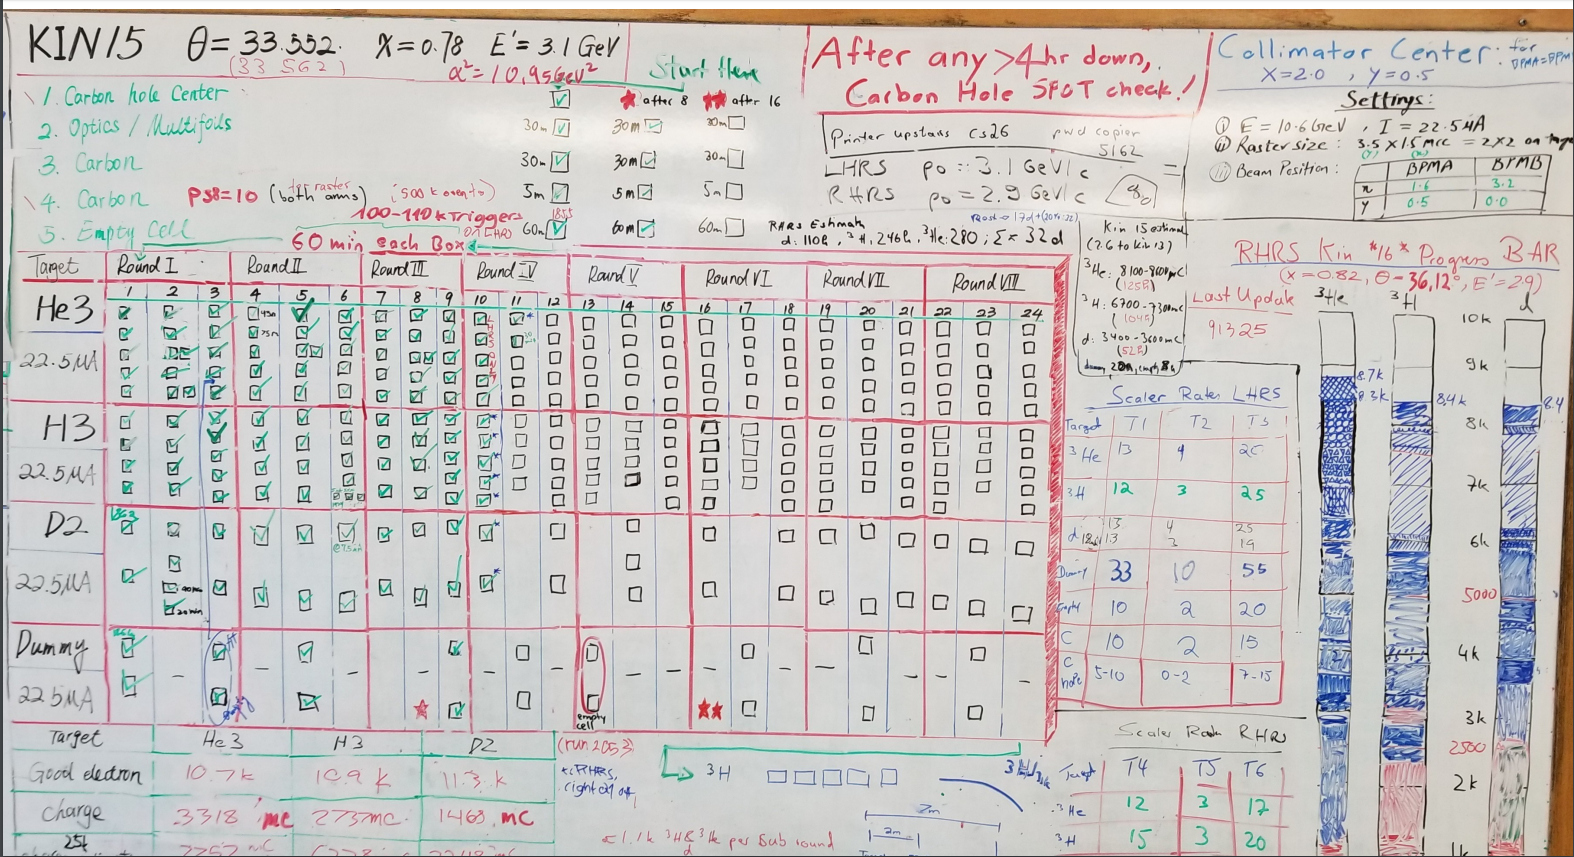
\includegraphics[width=6.5cm]{../images/whiteboard_2_20}
\end{figure}
\end{frame}

\begin{frame}
\frametitle{Kinematic Coverage}

\begin{figure}[h]
	\vspace*{-1.5cm}
	\centering
	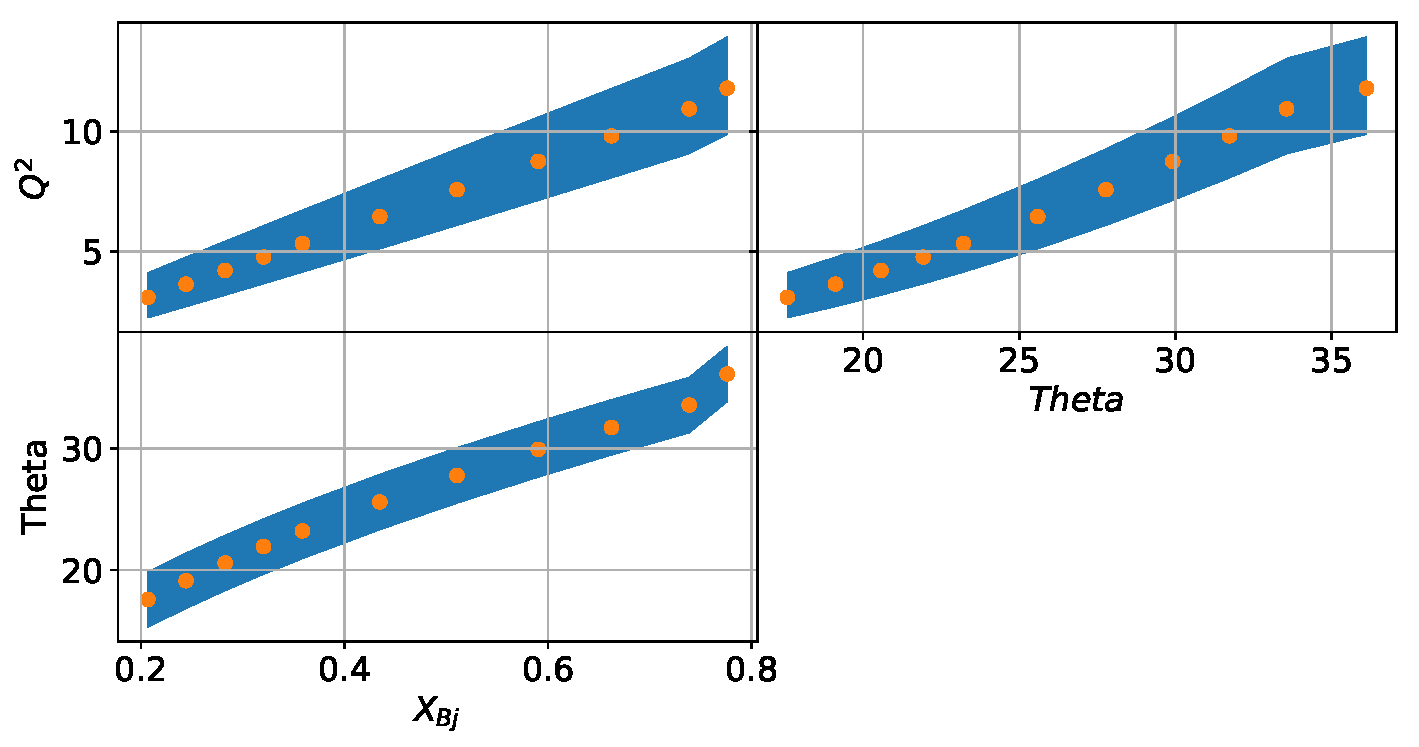
\includegraphics[width=12.cm]{../images/Thesis/KinCov.pdf}
	\caption*{Kinematic coverage between $Q^2$, $x$, and Theta. The band around the points represents the approximate spectrometer acceptance in the y axis.}
	\label{fig:kincov}
\end{figure}
\end{frame}
%------------------------------------------------------------------
\section[Analysis]{Data Analysis}
\begin{frame}
{\centering\huge{Path to The EMC Effect}}
%\vspace{10pt} 
\Large{
$\bullet$ Calibrate detectors to receive meaningful data\\
$\bullet$ Determine the yield, efficiency and background\\
$\bullet$ Calculate the cross sections and ratios\\
$\bullet$ Extract the corrected EMC effect!
}
\end{frame}



\subsection[Calibration]{Calibration}
\begin{frame}
\textbf{Preparing Data for Analysis}
\begin{columns}[]
\column{0.55\textwidth}
\begin{block}{Calibration}
	\begin{itemize}
		\item[] \textbf{ADC calibration}
		\item Calorimeters, Scintillators, and \textbf{Cherenkov}
		\item[] \textbf{TDC calibration}
		\item Scintillators and VDC
		\item[] \textbf{Detector calibrations} 
		\item Beam Current Monitors 
		\item \textbf{Beam Position Monitors}
	\end{itemize}
\end{block}
\column{0.45\textwidth}
\begin{figure}
	\vspace*{-0.25cm}
	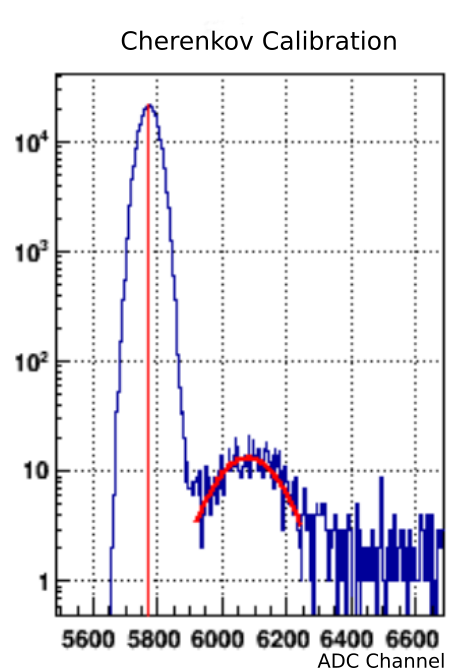
\includegraphics[width=5cm,height=6.5cm]{../images/gc_calib.png}
\end{figure}

\end{columns}
\end{frame}


\begin{frame}
\frametitle{Beam Position Monitor(BPM) Calibration}

	\begin{columns}
		\column{0.45\textwidth}
		\begin{figure}
			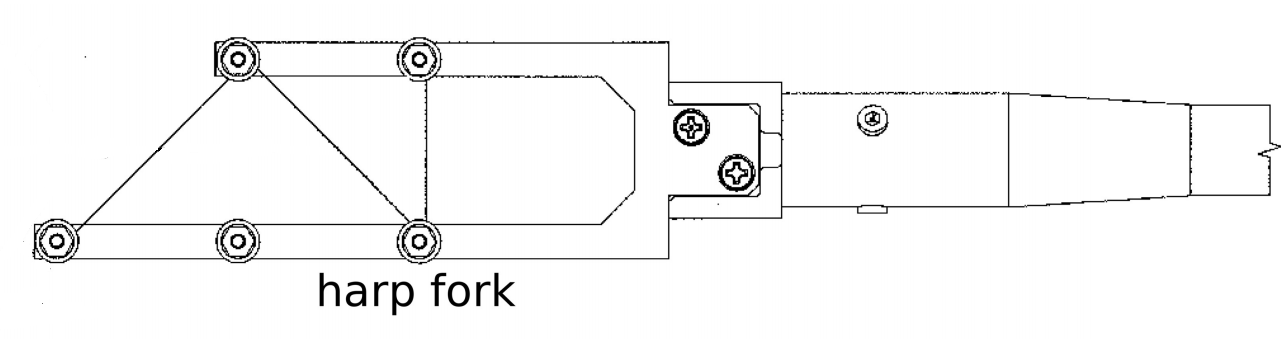
\includegraphics[width=5.5cm]{../images/Thesis/harp.png}
		\end{figure}
		Intrusive absolute position measurement
		\column{0.45\textwidth}
		\vspace{-15pt}
		\begin{figure}
			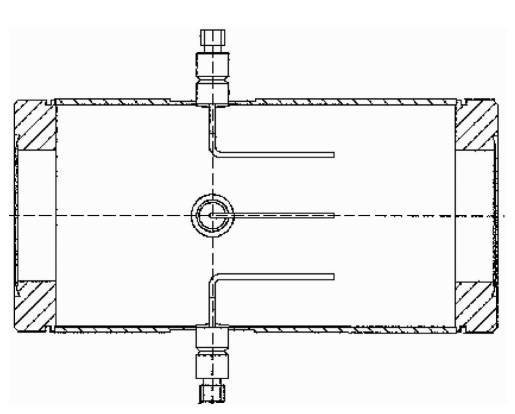
\includegraphics[width=3.5cm]{../images/Thesis/BPM.png}
		\end{figure}
		\vspace{-15pt}
		Relative position measurement
			
	\end{columns}	
		\centering
		\begin{equation}
			\begin{pmatrix}
			X_{position}\\
			Y_{position}
			\end{pmatrix}
			=
			\begin{pmatrix}
			C(0,0) & C(0,1)\\
			C(0,0) & C(0,1)\\
			\end{pmatrix}
			*
			\begin{pmatrix}
			X_{BPM}\\
			Y_{BPM}
			\end{pmatrix}
			+
			\begin{pmatrix}
			X_{offset}\\
			Y_{offset}
			\end{pmatrix}
			\nonumber			 
		\end{equation}
		
\end{frame}

\begin{frame}
\centering \textbf{Beam position from BPM and harp for a collection of runs}
\vspace*{-1cm}
\begin{columns}
	\column{0.5\textwidth}
\begin{figure}
	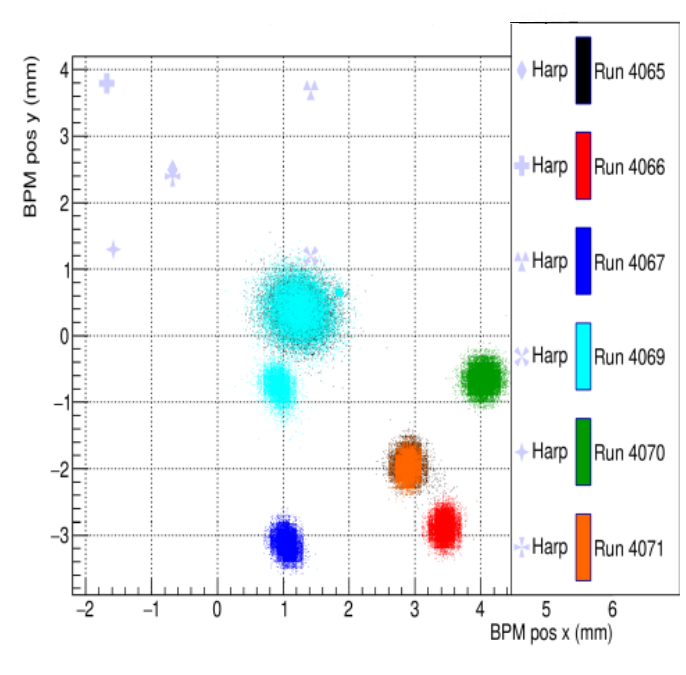
\includegraphics[width=6cm]{../images/BPM_before.png}
\end{figure}
\vspace*{-0.5cm}
\centering \textbf{Before Calibration} 
	\column{0.5\textwidth}
\begin{figure}
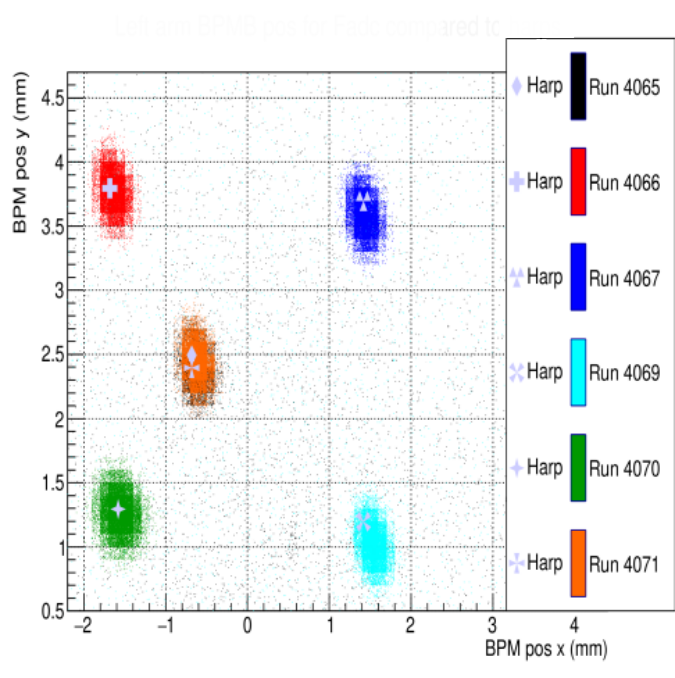
\includegraphics[width=6cm]{../images/BPM_after.png}
\end{figure}
\vspace*{-0.5cm}
\centering \textbf{After Calibration}
\end{columns}
\end{frame}

\subsection[Cross section]{Extracting Cross section}



\setlength{\blockheight}{.65\textheight}

\setlength{\blockwidth}{.95\textwidth}


\begin{frame}{Experimentally Measured Cross Section}

	%	\begin{columns}[c]
	%		\column{0.25\textwidth}
		\only<1,2,3,4,5,6>{
				\vspace*{-.95cm}
				\begin{figure}
					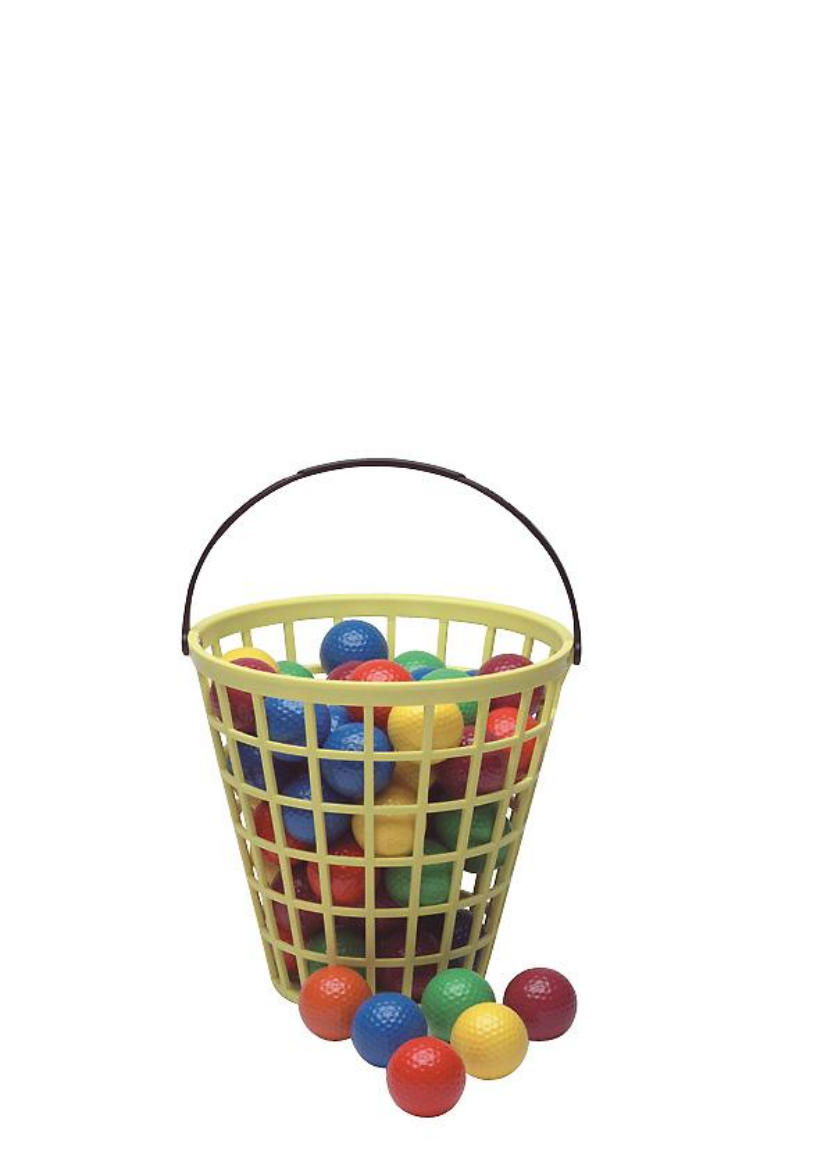
\includegraphics[width=3.cm]{../images/ballsinbucket.png}
				\end{figure}}
	%		\column{0.55\textwidth}
			\only<7->{
			%	\vspace{0.75cm}
				\begin{equation}
					\dfrac{d\sigma}{dE^{\prime}d\Omega} = \frac{(N - BG)}{L \cdot \epsilon \cdot \Delta E^{\prime} \Delta \Omega \cdot A(E^{\prime},\theta)} \nonumber
				\end{equation}
				\vspace{0.75cm}
			}
	%	\end{columns}
\vspace*{-1.15cm}
		\begin{itemize}
			\begin{columns}[t]
				\column{0.45\textwidth}
					\onslide<2->{\item N = Number of electrons}
					\onslide<5->{\vfill \item BG = Background}
					\onslide<2->{\vfill \item L = Luminosity }
					\vspace{-10pt}
					\begin{itemize}
						\onslide<3->{\item Density Correction }
					\end{itemize}
				\column{0.45\textwidth}
					\onslide<4->{\item $\epsilon$ = Efficiency }
					\onslide<6->{\item $\Delta E^{\prime} \Delta \Omega$= Bin Size }
					\onslide<6->{\item $A(E^{\prime},\theta)$ = Acceptance probability }
			\end{columns}
		\end{itemize}

\end{frame}


\begin{frame}
\begin{block}{Efficiencies ($\epsilon$)}
	\begin{columns}[t]
		
				\column{0.45\textwidth}	
		\onslide<1->	Calculating efficiencies
		\begin{itemize}
			\onslide<2->\item Use well defined samples from separate system(s)
			
						\onslide<3->{
				\begin{itemize}
				\item Testing cherenkov use calorimeters
				\item Testing VDC use scintillators. 				\end{itemize}						}
			\onslide<4->\item Determine good event samples with cuts
			\onslide<5->\item \# of events which fail the criteria $\rightarrow$ inefficiency 
		\end{itemize}
		
		
		
		\column{0.45\textwidth}
		\begin{itemize}

			
		\onslide<6->{	\item Particle Identification(PID) 
			\begin{itemize}
				\item Cherenkov
				\item Calorimeters
			\end{itemize}}
		\onslide<7->{	\item Trigger
			\begin{itemize}
				\item Scintillators \& cherenkov
				\item $\approx$ 99\%
			\end{itemize}}
		\onslide<8->{	\item Tracking
			\begin{itemize}
				\item Vertical Drift Chambers(VDCs)
				\item $\approx$ 98\%
			\end{itemize}}
		\onslide<9->{	\item Electronic Deadtime
			\begin{itemize}
				\item $\approx$ 96\%-99\%
			\end{itemize}}
		\end{itemize}

		
	\end{columns}
\end{block}
\end{frame}

\begin{frame}{}
\frametitle{Particle ID Efficiency}
\begin{columns}
\column{0.65\textwidth}
\begin{figure}[t]%
	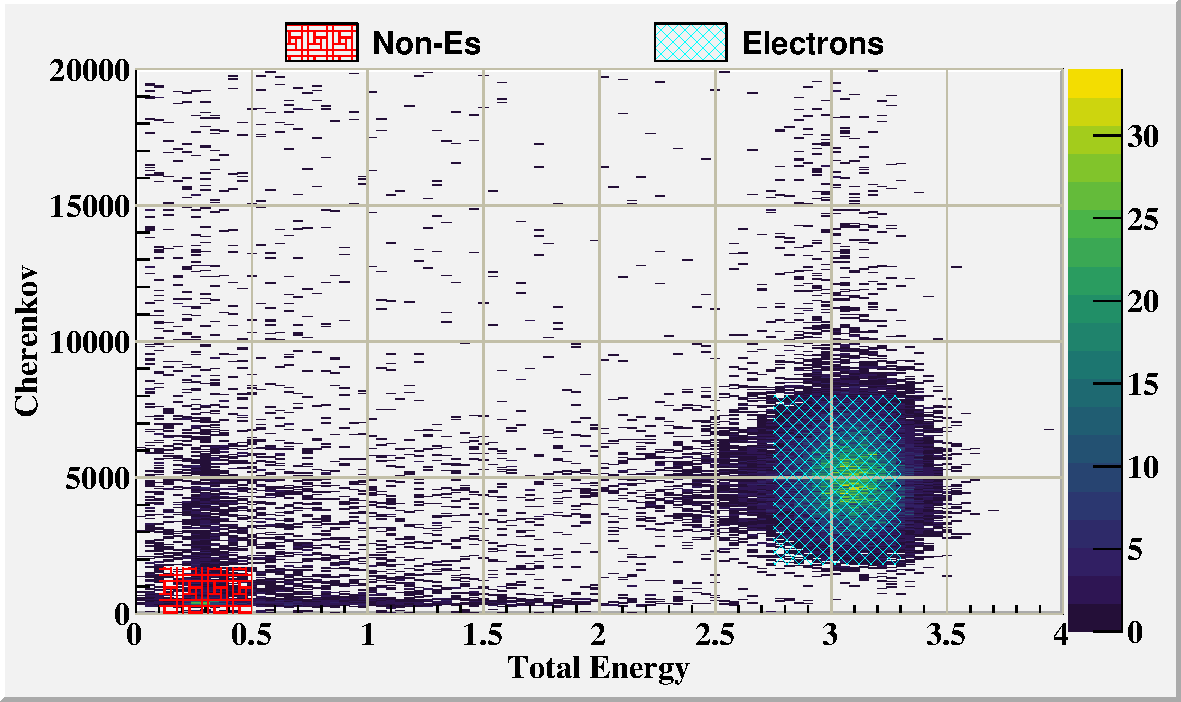
\includegraphics[width=8cm]{../images/Thesis/PID_2d}
\end{figure}
\column{0.35\textwidth}
\begin{itemize}
	\item Total energy absorber for electrons
	\item Cherenkov's pion threshold is $>$ momentum setting
	\item PID efficiency $\approx 98\%$  for all kinematics 
\end{itemize}

\end{columns}	
\end{frame}

\subsection[Systematic Studies]{Systematic Studies}
%------------------------------------------------------------------

\begin{frame}{Charge Symmetric Background}
\vspace{-0pt}

\begin{columns}
	\column{0.55\textwidth}
	\vspace*{-0.75cm}
	\begin{itemize}
		\item $\gamma$ decay into an e$^+$e$^-$ pairs
		\item  Pair produced $e^-$ by detecting e$^+$
		\item Extraction based on fit to Exponential function 
	\end{itemize}
	\column{0.45\textwidth}
	\vspace{-40pt}
	\begin{figure}
		\textbf{Pair Production}
		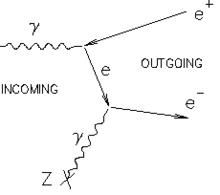
\includegraphics[width=3.0cm]{../images/pp_FD.png}
	\end{figure}
\end{columns}


\begin{figure}
	\caption*{Tritium positron contamination. Credit: Tong Su}
	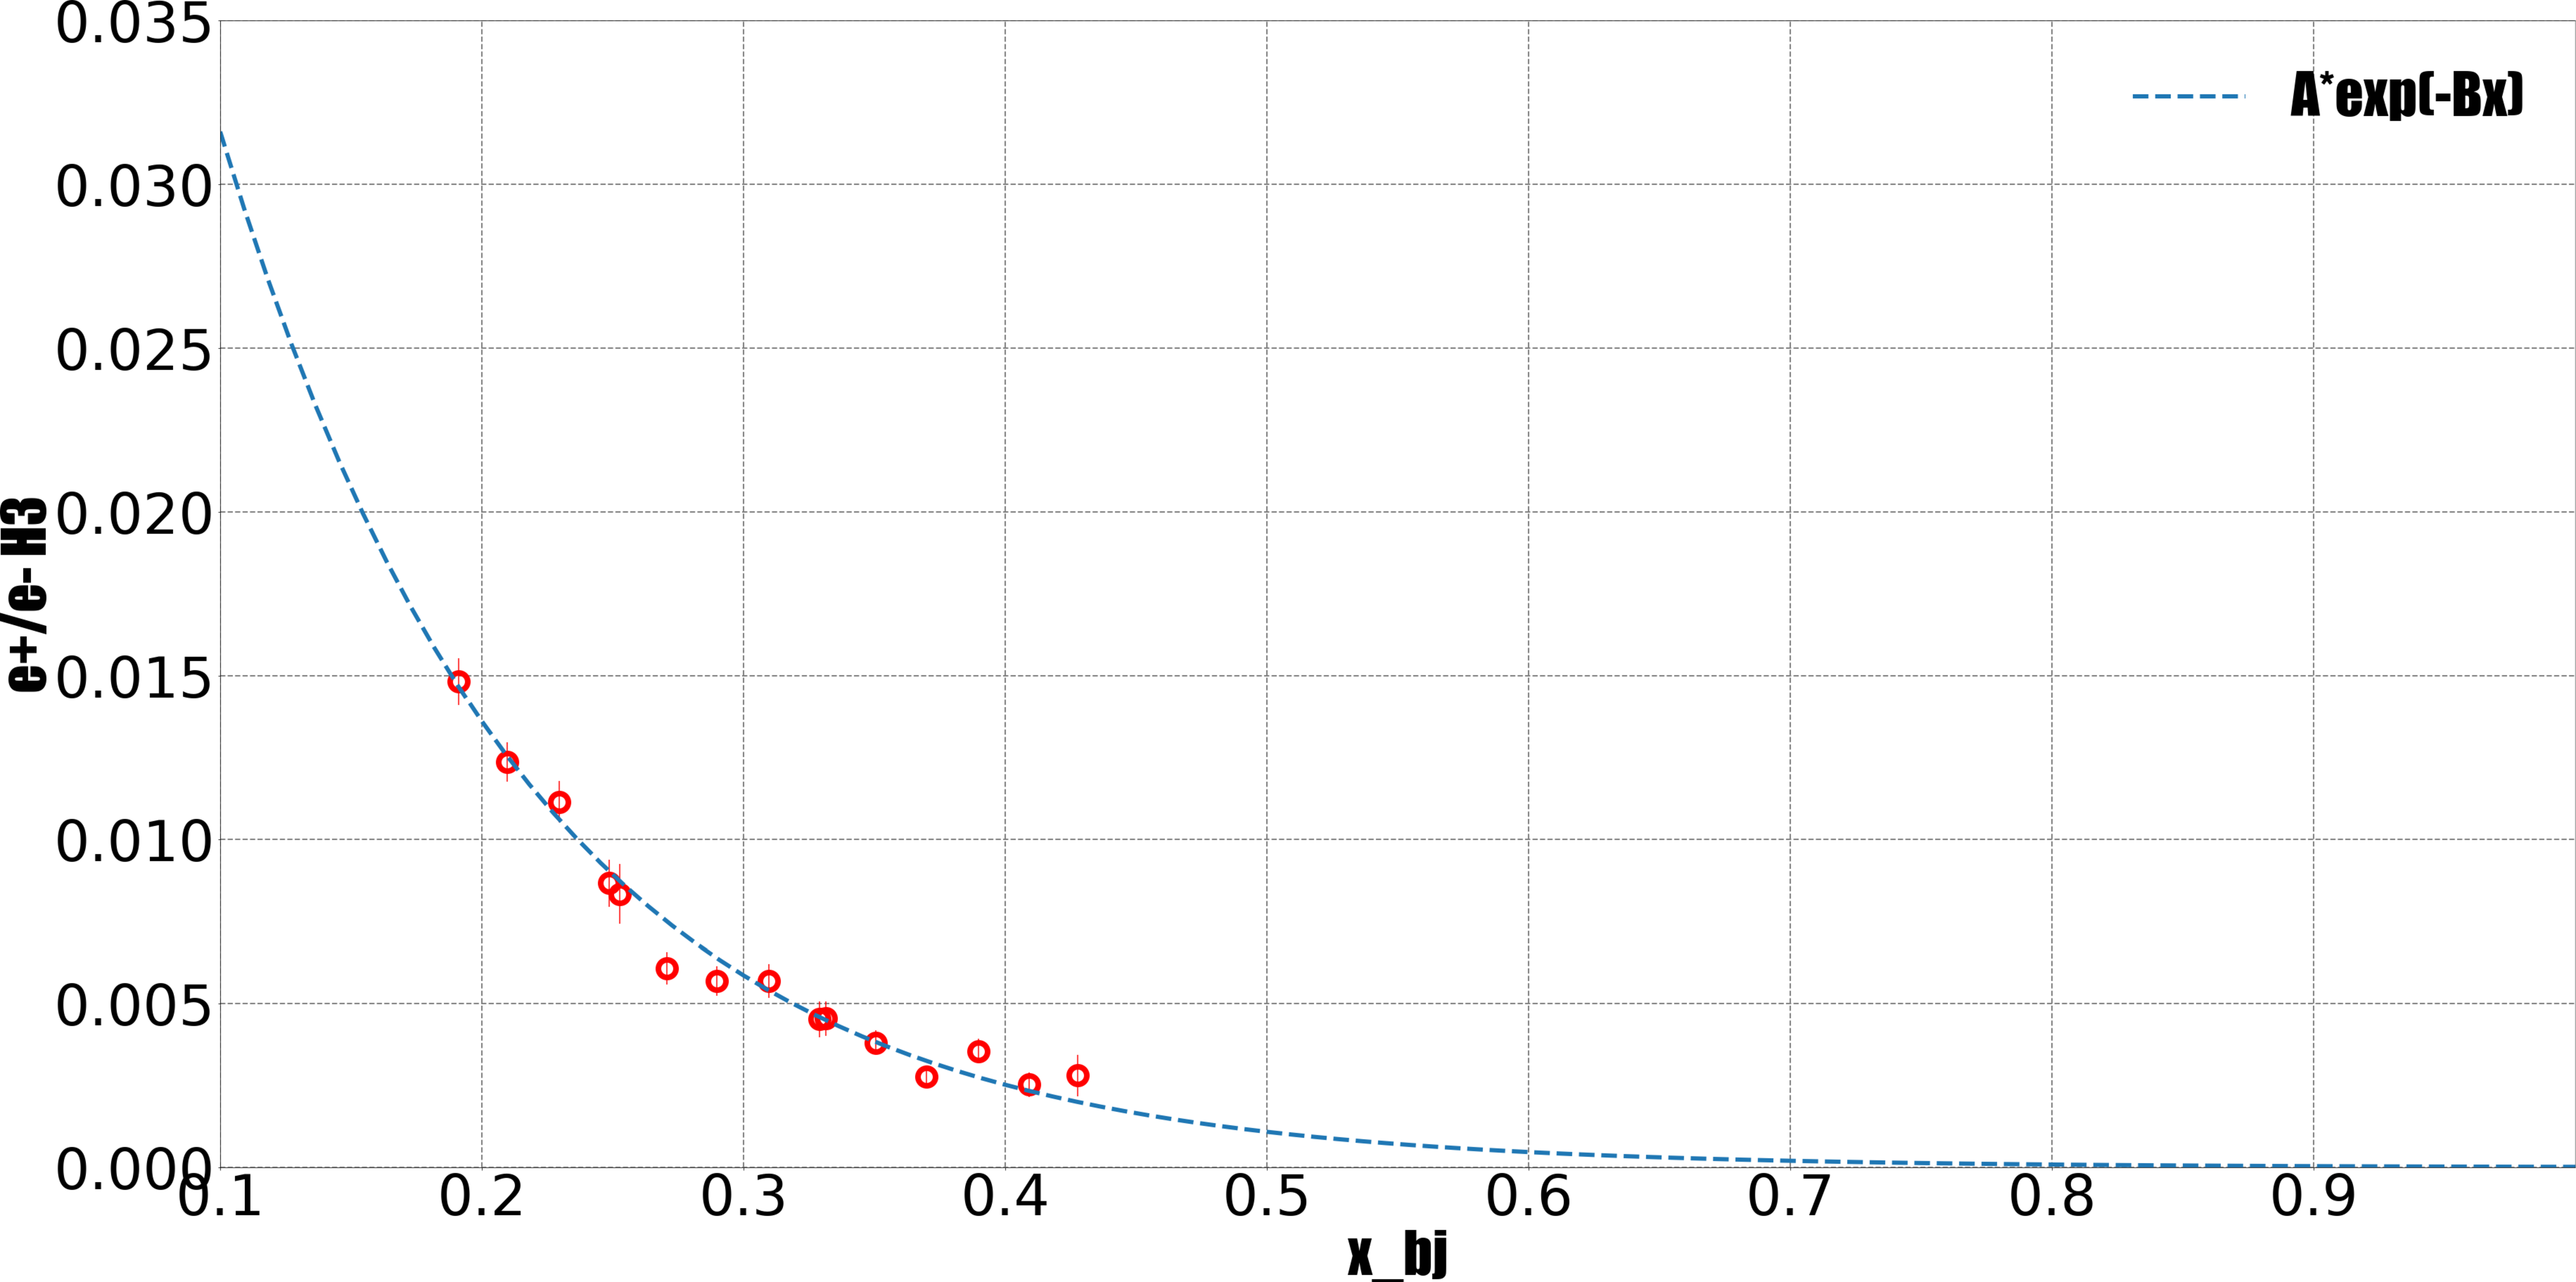
\includegraphics[width=8.0cm]{../images/positron_H3_bane.pdf}
\end{figure}




\end{frame}

\begin{frame}
\frametitle{Aluminum Endcap Background}
	\vspace{-15pt}
\begin{block}{}
	\begin{figure}
		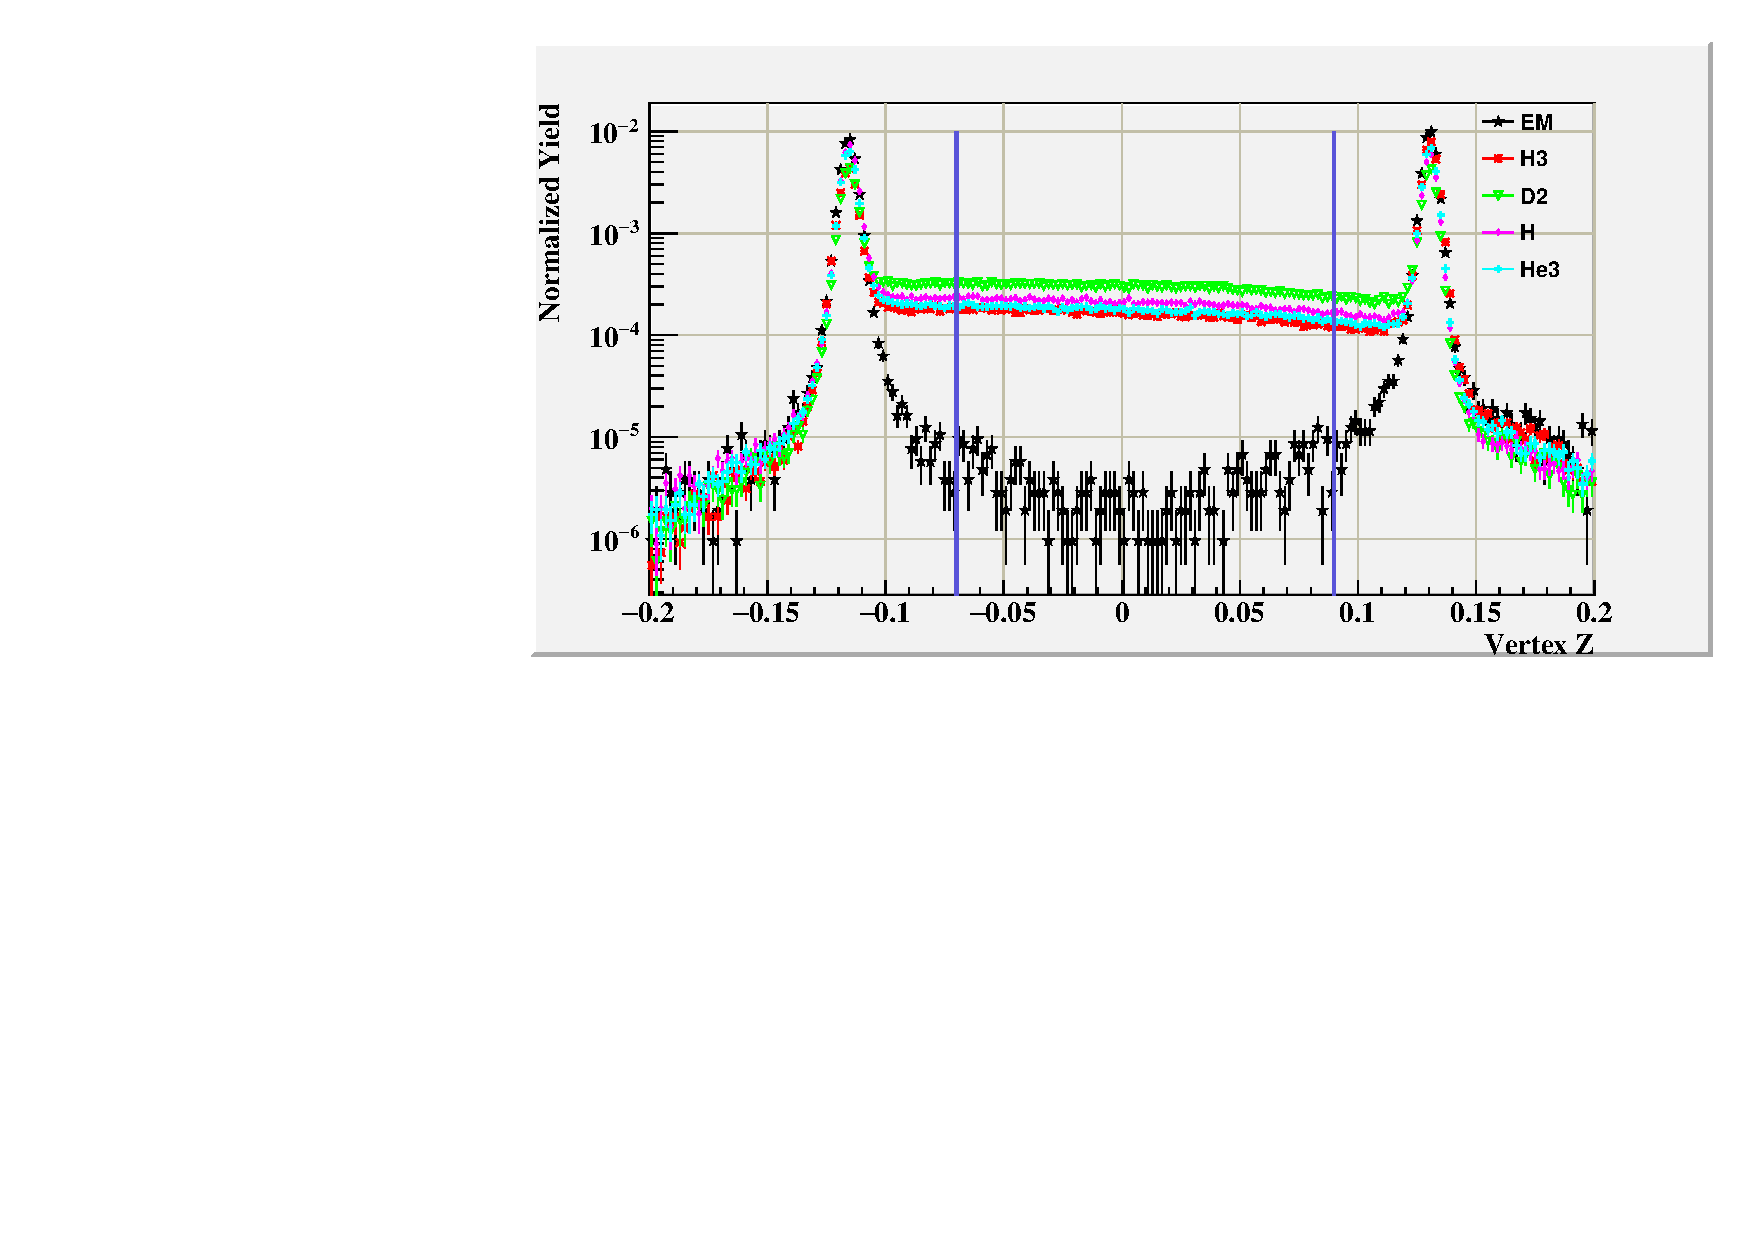
\includegraphics[width=11.0cm]{../images/endcap_kin4.pdf}
	\end{figure}

\begin{itemize}
	\item Extract ratio of the normalized yield from the gas cell to that of the empty cell
\end{itemize}

\end{block}
\end{frame}
%------------------------------------------------------------------em_tgt_comp.png

\begin{frame}
\frametitle{$^3H $ Decay}
\begin{block}{$^3H \rightarrow ^3He$}
	\begin{columns}
		\column{0.45\textwidth}
		\begin{equation*}
		\tau(^3H) = 4500 \pm 8 days
		\end{equation*}		 	
		\\
		\begin{equation*}
		c = \frac{\eta_{^3He}} {\eta_{tot}}
		\end{equation*}
		\\
		\begin{equation*}
		\sigma_{^3H} = \big(\frac{\sigma_{tot}}{\sigma_{^3He}}\big) \big(\frac{1}{1-c}\big) -  \big(\frac{1}{1-c}\big)  
		\end{equation*}
		\column{0.55\textwidth}
		\begin{figure}
			\caption*{Beta Decay Helium Fraction}
			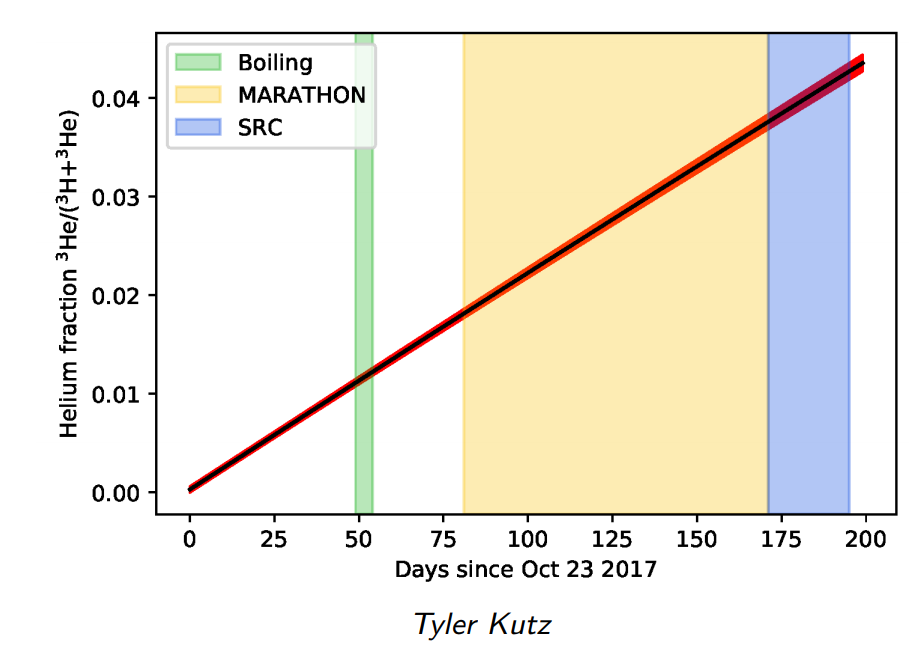
\includegraphics[width=6cm]{../images/beta_decay.png}
		\end{figure}
	\end{columns}
\end{block}
\end{frame}



%------------------------------------------------------------------


\begin{frame}{Density Fluctuations}
	\vspace{-17pt}
	\begin{figure}
		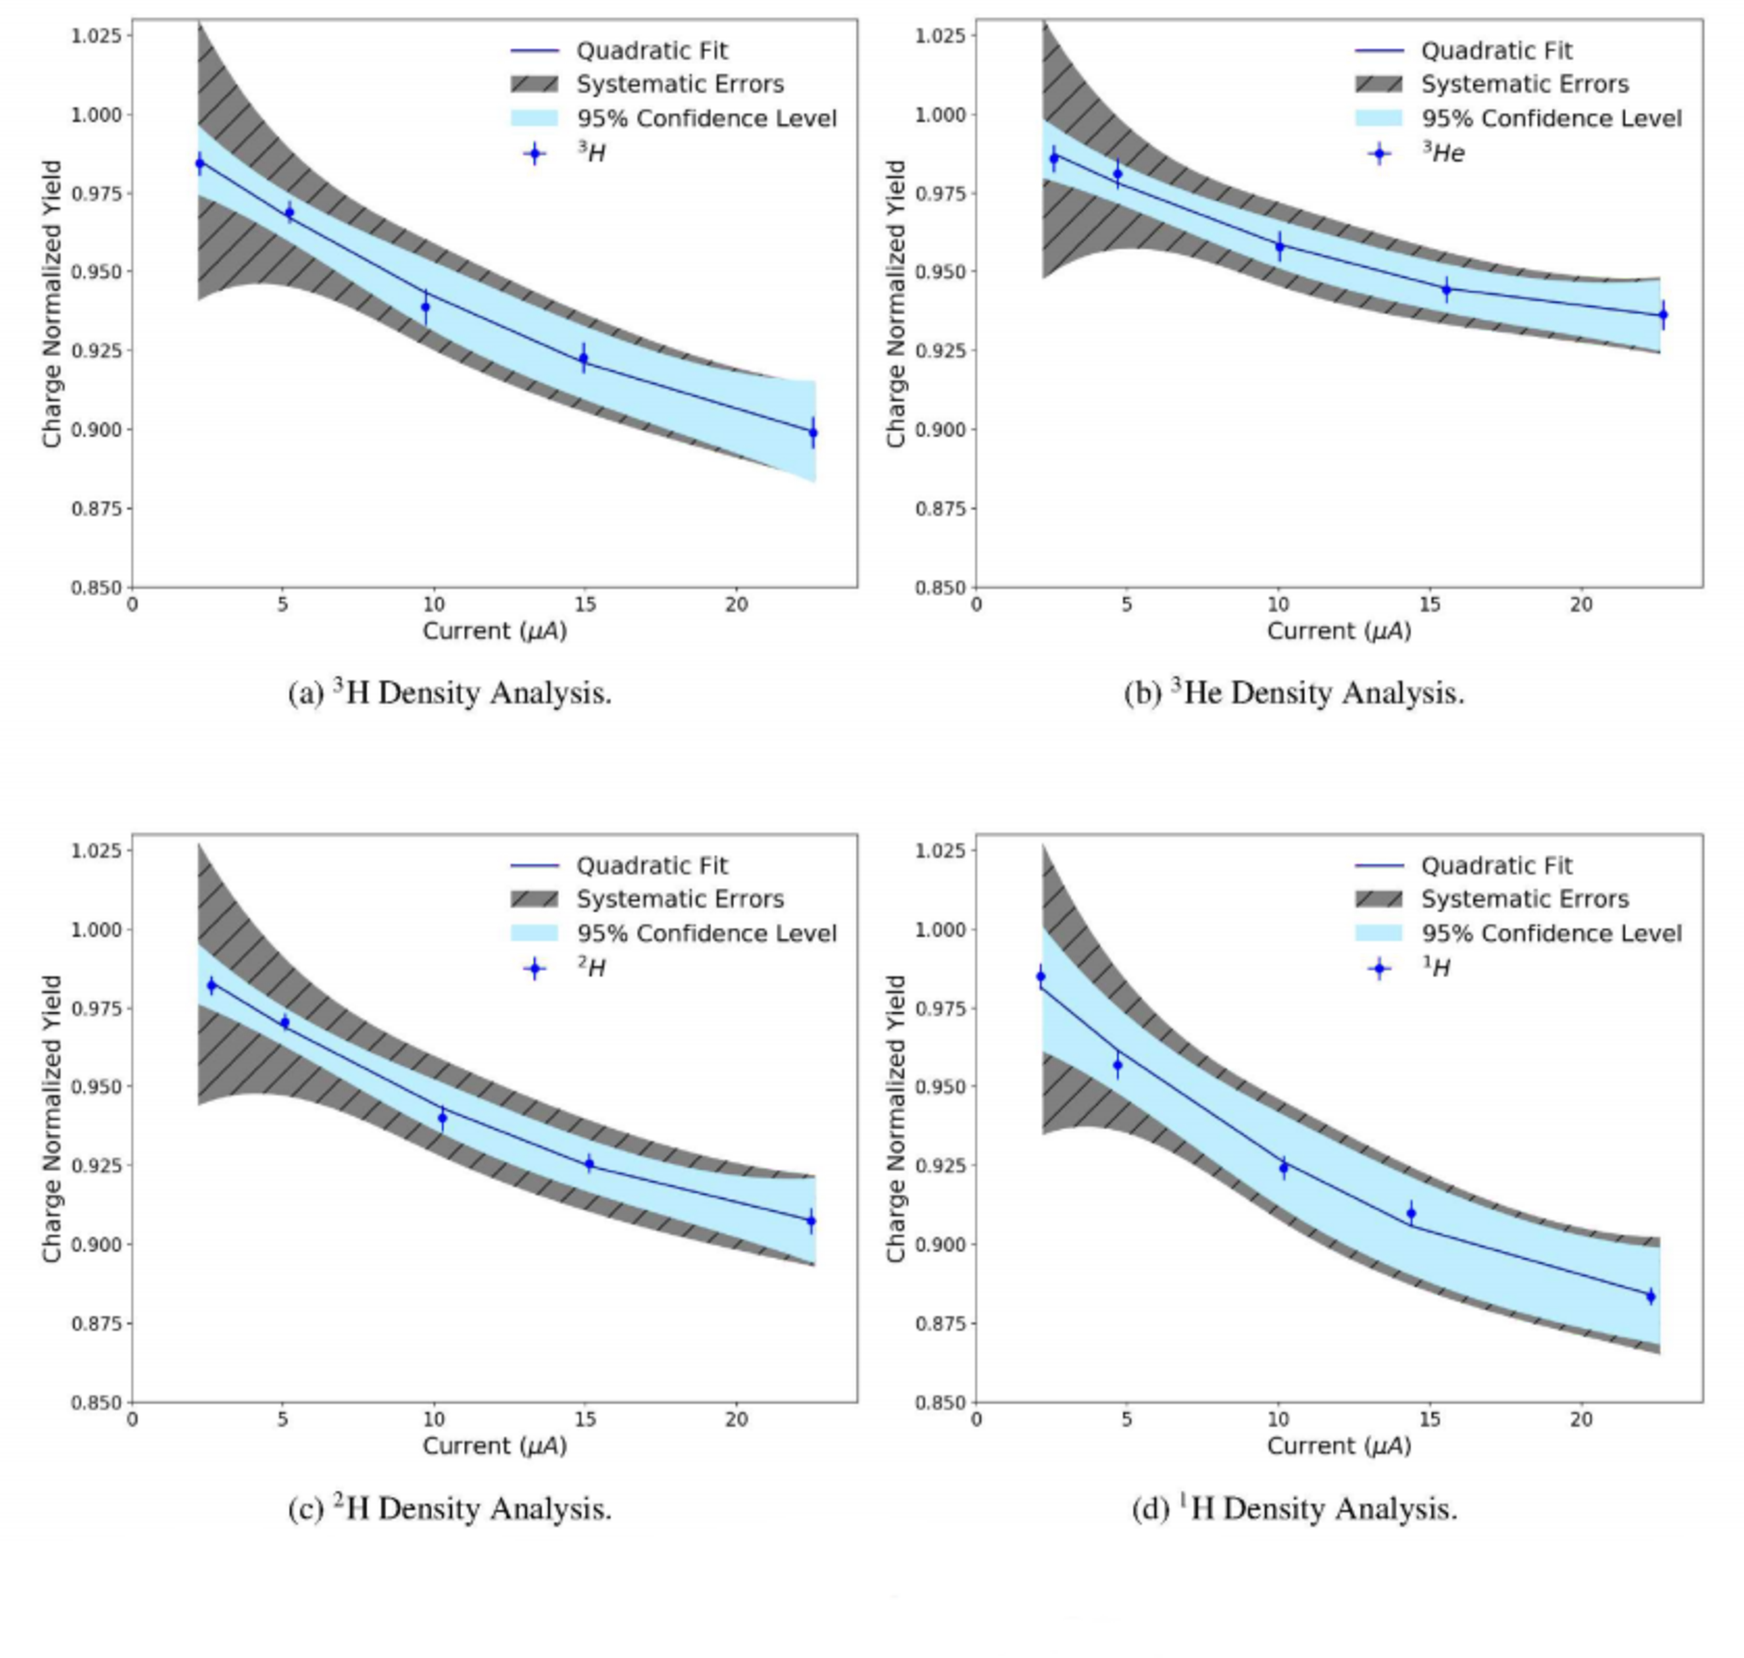
\includegraphics[width=10cm,height=7.50cm]{../images/density_cor.pdf}
		\vspace{-0.5cm}
		\caption*{\footnotesize{S.N. Santiesteban, J. Bane, et. al \emph{Nucl. Instrum. Meth. A} 940 (2019) 351-358} }
	\end{figure}

\end{frame}

\begin{frame}
	\begin{block}{Monte Carlo Ratio Method}
	\begin{equation}
		\sigma_{Data} = \frac{Y_{data}(E^{\prime},\theta)}{ L \cdot (\Delta E^{\prime} \Delta 
		\Omega) \cdot A(E^{\prime},\theta) }\nonumber
	\end{equation}
		\onslide<2->{
			\begin{equation}
				Y_{MC}(E^{\prime},\theta) = L \cdot \sigma^{model} \cdot (\Delta E^{\prime} \Delta \Omega) \cdot A(E^{\prime},\theta) \nonumber
			\end{equation}
		}
	\onslide<3->{Use a Monte Carlo simulation  \\}
	\onslide<4->{$\bullet$ $(\Delta E^{\prime} \Delta \Omega)_{Data}$ =$(\Delta E^{\prime} \Delta \Omega)_{MC}$\\ }
	\onslide<4->{$\bullet$ $A(E^{\prime},\theta)_{Data} = A(E^{\prime},\theta)_{MC}$}
	\onslide<5->{
	\begin{equation}
		\sigma_{Data} = \sigma_{model} \cdot \frac{Y_{Data}}{Y_{MC}}\nonumber
	\end{equation}} 
	\end{block}
\end{frame}



%------------------------------------------------------------------
\begin{frame}{}
\begin{columns}
	\column{0.5\textwidth}
	\begin{block}{Monte Carlo}
		\begin{itemize}
			\item Generate events $\rightarrow$ Pass through magnetic apertures
			\item Tune Simulation offsets to match detector response
			\item Use model to weight events
			\begin{itemize}
				\item Deep Inelastic and resonance region from Ari Bodek Fit from E139 
				\item Full Mo and Tsai radiative correction
			\end{itemize}
		\end{itemize}
		\cite{bodek}  
		[L.W. Mo and Y.S. Tsai, 1969] 
	\end{block}
	\column{0.45\textwidth}
	\vspace{-20pt}
	\begin{figure}
		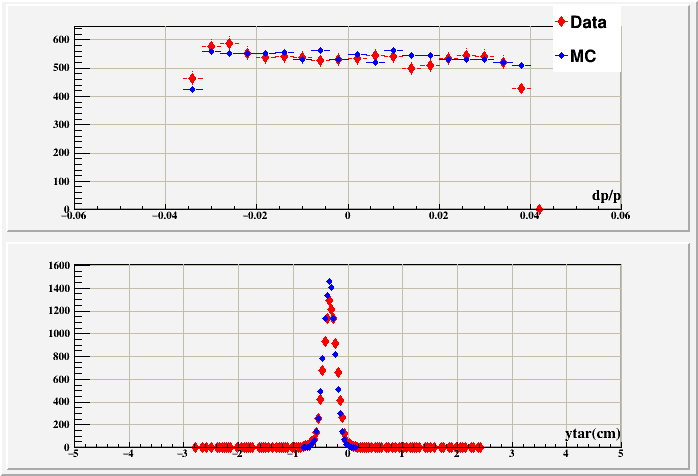
\includegraphics[width=6cm]{../images/dp_ytar_1207.png}
	\end{figure}
	\vspace{-30pt}
	\begin{figure}
		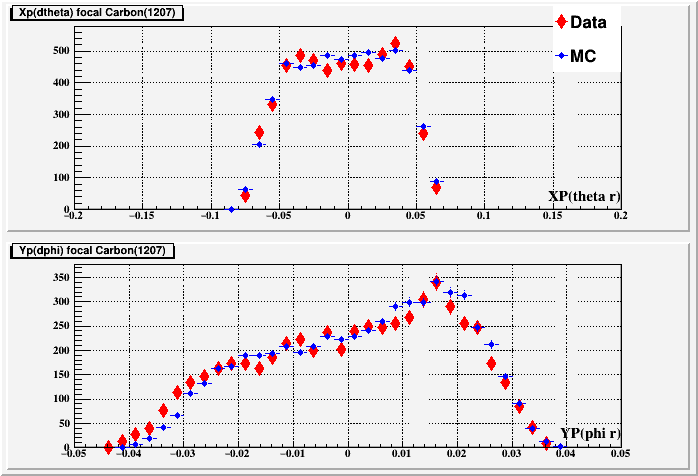
\includegraphics[width=6cm]{../images/xp_yp_foc_1207.png}
	\end{figure}
\end{columns}
\end{frame}



\subsection[Results]{Results}
\begin{frame}
\Huge{Result}\\
\Large{Deep Inelastic Cross Section}\\
\qquad 10.6 GeV Beam, W$^2$ $>$ 3.5 Gev$^2$\\
\qquad Scatted angles 17.5$^\circ$ to 31$^\circ$\\
\Large{Cross Section Ratios}\\
\Large{EMC Effect}
\Large{First DIS cross section and EMC measurement of $^3H$}
\Large{First direct comparison of two A=3 EMC effects.}


\end{frame}

\begin{frame}{}
\frametitle{DIS Cross Section}
\centering
\vspace{-20pt}
\begin{figure}
	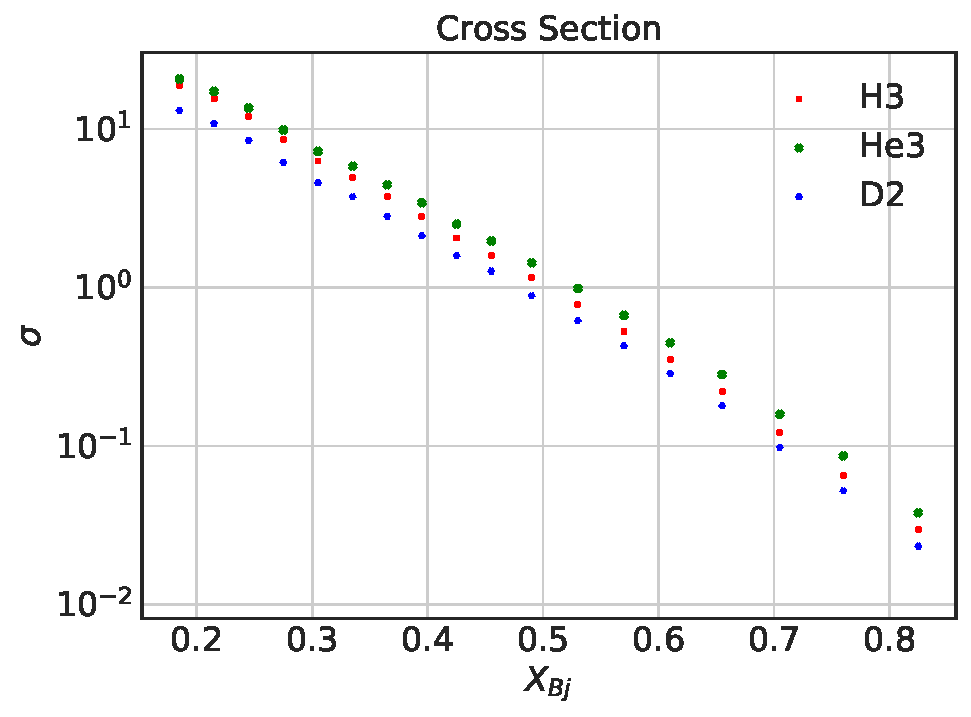
\includegraphics[width=11cm]{../images/Thesis/total_xs.pdf}
\end{figure}

Normalization uncertainty due to target thickness uncertainty\\
$^3$He - 1.12$\%$ $\bullet$ $^3$H - 0.97$\%$ $\bullet$  D - 0.56$\%$
\end{frame}
%----------------------------------------------
\begin{frame}{}

\begin{table}[]
	\caption*{Relative Error Contributions for the Cross Section $^3$H.}
	\begin{tabular}{|p{2.2cm}|l|l|l|l|l|l|}
\hline
\multicolumn{1}{|r|}{\textbf{Xbjc}} & \textbf{0.185} & \textbf{0.305} & \textbf{0.49} & \textbf{0.57} & \textbf{0.705} & \textbf{0.825} \\ \hline
\textbf{Yield Error}                & 0.01           & 0.0107         & 0.0149        & 0.0151        & 0.0141         & 0.0163         \\ \hline
Stat Error*                         & 0.0055         & 0.0059         & 0.01          & 0.0111        & 0.0113         & 0.0143         \\ \hline
End Cap*                            & 0.007          & 0.007          & 0.007         & 0.007         & 0.007          & 0.007          \\ \hline
Eff Error*                          & 0.004          & 0.0051         & 0.0083        & 0.0071        & 0.0041         & 0.0032         \\ \hline\hline
\textbf{MC\&Model}                  & 0.016          & 0.014          & 0.013         & 0.016         & 0.03           & 0.037          \\ \hline
Resolution**                        & 0.015          & 0.011          & 0.005         & 0.001         & 0.007          & 0.018          \\ \hline
Model**                             & 0.006          & 0.009          & 0.012         & 0.016         & 0.029          & 0.032          \\ \hline\hline
\textbf{Total Error}                & 0.019          & 0.018          & 0.02          & 0.022         & 0.033          & 0.04           \\ \hline
\end{tabular}

	* Largest contributers to the error in the yield calculation\\
	** Largest contributers to the error in Monte Carlo and Cross section model calculation. 

\end{table}


\end{frame}
%----------------------------------------------
\begin{frame}{}
\frametitle{Per Nucleon Cross Section Ratio}
\vspace{-20pt}
\begin{figure}
	\includegraphics[width=11cm]{../images/Thesis/A_D_ratios.pdf}
	\caption*{MARATHON results compared with E03103 \cite{E3103} and the A/D ratios from a DIS scattering model from Arie Bodek model \cite{bodek}.}
\end{figure}

\end{frame}

%----------------------------------------------
\begin{frame}{}
\frametitle{Isoscalar Corrections}
\vspace*{-1cm}
\begin{columns}
	\column{0.5\textwidth}
	\begin{figure}
		\includegraphics[width =5cm]{../images/mirror}
	\end{figure}
	\column{0.5\textwidth}
	$\bullet$ Correct for the unpaired nucleon in the A/D ratio.	
\end{columns}
\begin{equation}
F^A_{Iso} = \frac{\Big(0.5*(1.0 + \frac{F_2^n}{F_2^p})\Big)}{ \Big(\frac{1}{A} \cdot \big(Z+(A-Z)\cdot \frac{F_2^n}{F_2^p}\big) \Big) }\nonumber
\end{equation}

\end{frame}

%----------------------------------------------
\begin{frame}{}
\frametitle{Isoscalar Corrections}
\vspace*{-0.75cm}

\begin{figure}
	\includegraphics[width =11cm]{../images/Thesis/ISOfacs1.pdf}
	\caption*{Isoscalar correction factor for both $^3$He and $^3$H. Model dependent calucation, error is calcualted via comparing different models for $\frac{F_2^n}{F_2^p}$.}
\end{figure}

\end{frame}
%----------------------------------------------
\begin{frame}{}
$\bullet$ My EMC results for \textcolor{black}{He3 in black} \textcolor{red}{$\bullet$ H3 in red}\\
$\bullet$ \textcolor{ForestGreen}{Previous Jlab He3 in green}
\begin{figure}
	\includegraphics[width=10cm]{../images/Thesis/EMC_ratios.pdf}
	\caption*{MARATHON results compared with E03103 \cite{E3103} and the EMC ratios from a DIS scattering model from Arie Bodek model \cite{bodek}.}
\end{figure}
\end{frame}

\begin{frame}{Ratio of $^3$H/$^3$He EMC effects}
\vspace{-20pt}
\begin{figure}
	\includegraphics[width=12cm]{../images/Thesis/A_ratios.pdf}
	\caption*{Ratio of EMC effects. Black is Isoscalar correct, red is not. }
\end{figure}
\end{frame}



\begin{frame}{}
\begin{block}{Summary}
	\begin{itemize}
		\item Used DIS to extract inclusive cross section for $^3$H, $^3$He, and D
		\item Looked at the A/D ratio for both $^3$H and $^3$He
		\item Applied model dependent correction for excess protons and neutrons.
		\item Compared the EMC effects of the two, A=3 nuclei. 
		\begin{itemize}
			\item See no difference for Isoscalar EMC effects within analysis accuracy
		\end{itemize}
	\end{itemize}
\centering
%\large{Understanding the effect of neutron/proton excess on the EMC Effect}
\end{block}

\begin{figure}
	\includegraphics[width =5cm]{../images/puzzle2.png}
\end{figure}

\end{frame}


%----------------------------------------------
\section{Future Experiments}
\begin{frame}{}

\small{\textbf{Detailed Studies of the nuclear dependence of F2 in light nuclei 
	[E12-100-008: J. Arrington, A Daniel, NF, D. Gaskell]}}
\begin{figure}
	\includegraphics[width=10cm]{../images/moreEMC.png}
	\caption*{Slide credit Nadia Fomin}
\end{figure}
\end{frame}
%----------------------------------------------
\begin{frame}{}

\centering \textbf{The EMC effect in spin structure functions}
\begin{figure}
	\includegraphics[width=10cm]{../images/moreEMC1.png}
	\caption*{Slide credit Nadia Fomin}
\end{figure}

\end{frame}
%----------------------------------------------
\begin{frame}{}
\begin{block}{Special Thanks}
	\begin{itemize}
		\item The Tritium Students 
		\item JLab staff and technicians
		\item Nadia Fomin and Douglas Higinbotham
		\item DOE and JSA(Jefferson Science Associates)
	\end{itemize}
\end{block}
\end{frame}






\begin{frame}[allowframebreaks]
\vspace*{-3pt}
\frametitle{References}
\footnotesize{
	\begin{thebibliography}{9} % Beamer does not support BibTeX so references must be inserted manually as below
		\vspace*{-20pt}
		\bibitem[J.J. Aubert, et al. 1981]{cc} J.J. Aubert, et al.
		\newblock \emph{Phys.Lett. 105B (1981) 315-321 CERN-EP/81-84}
		\vspace*{-8pt}		
		\bibitem[A. Bodek and U.K. Yang, 2002]{bodek} A. Bodek and U.K. Yang
		\newblock \emph{Nuclear Physics B, Procc. Suppl. 112 (2002) 70-76 }			
\vspace*{-8pt}
		 \bibitem[Bickerstaff and Thomas, 1989]{EMC_model_1} R~P Bickerstaff and A~W Thomas.
\newblock The {EMC} effect-with emphasis on conventional nuclear corrections.
{\em Journal of Physics G: Nuclear and Particle Physics},
15(10):1523--1569, oct 1989.
\vspace*{-8pt}

		 \bibitem[Cloet, and Thomas, 2006]{EMC_medium_1}
I.~C. Cloet, W.~Bentz, and A.~William Thomas.
\newblock {EMC and polarized EMC effects in nuclei}.
{\em Phys. Lett.}, B642:210--217, 2006.
\vspace*{-8pt}
%		\bibitem[P. Bosted and E. Christy]{F1F} Bosted $\&$ Christy (2008)
%		\newblock Phys. Rev. C 77, 065206 (2008)
		\bibitem[G. T. Garvey, et al., 2015]{spectrum} Garvey, G. T. et. al.
		\newblock \emph{Phys. Rept., 580 (2015) 1-45 }	
\vspace*{-8pt}		
		 \bibitem[Geesaman, Saito, and Thomas, 1995]{Geesaman}  D.F. Geesaman, K~Saito, and A~Thomas.
		\newblock The Nuclear EMC Effect. {\em Annual Review of Nuclear and Particle Science}, 45(1):337--390,
		1995.
		
\vspace*{-8pt}		
		\bibitem[J. Gomez et al., 1994]{slac_emc} J. Gomez et al.   
		\newblock \emph{Phys. Rev D}  49 (1994) 4348 

\vspace*{-8pt}		
		\bibitem[K. Nakamura et. al. 2010]{Rev_PP} K. Nakamura et. al.
		\newblock \emph{Review of Particle Physics, 37 (2010) }	
\vspace*{-8pt}
		\bibitem[Norton, 2003]{Norton} P~R Norton.
\newblock The EMC Effect.{\em Reports on Progress in Physics}, 66(8):1253, 2003.
\vspace*{-8pt}		
		\bibitem[S.N.Santiesteban et. al (2019)]{denscor} S.N.Santiestebana et. al 
		\newblock 	\emph{Nucl. Instrum. Meth.} A 940 (2019) 351-358
\vspace*{-8pt}				
		\bibitem[J.Seely, A. Daniel et al, 2009]{E3103} J. Seely, A. Daniel et al  
		\newblock \emph{Phys.\ Rev.\ Lett.\   103, 202301 (2009)}.
\vspace*{-8pt}
		\bibitem[Smith and Miller, 2007]{EMC_medium_2} J.~R. Smith and G.~A. Miller
\newblock {Chiral solitons in nuclei: Saturation, EMC effect and Drell-Yan
	experiments}.
{\em Phys. Rev. Lett.}, 91, 2003. Erratum: {\em Phys. Rev. Lett}, 98, 2007.
\vspace*{-8pt}				
		\bibitem[Povh, 1995]{PnN} Bogdan Povh,
		\newblock Particles and Nuclei: An Introduction to the Physical Concepts, (1995)
			
	


		 

		 



	\end{thebibliography}
}
\end{frame}

\backupbegin
\begin{frame}
\centering
\LARGE{Backup Slides}

\end{frame}


%----------------------------------------------
\begin{frame}{}

\begin{table}[]
	\caption*{Relative Error Contributions for the Cross Section $^3$He.}
	\begin{tabular}{|p{2.2cm}|l|l|l|l|l|l|}
\hline
\multicolumn{1}{|r|}{\textbf{Xbjc}} & \textbf{0.185} & \textbf{0.305} & \textbf{0.49} & \textbf{0.57} & \textbf{0.705} & \textbf{0.825} \\ \hline
\textbf{Yield Error}                & 0.0104         & 0.011          & 0.0147        & 0.0149        & 0.0139         & 0.0161         \\ \hline
Stat Error*                            & 0.0063         & 0.0064         & 0.0098        & 0.0108        & 0.0111         & 0.0141         \\ \hline
End Cap*                             & 0.007          & 0.007          & 0.007         & 0.007         & 0.007          & 0.007          \\ \hline
Eff Error*                           & 0.004          & 0.0051         & 0.0083        & 0.0071        & 0.0041         & 0.0031         \\ \hline
\hline
\textbf{MC\&Model}                  & 0.016          & 0.017          & 0.012         & 0.013         & 0.033          & 0.024          \\ \hline
Resolution**                          & 0.015          & 0.012          & 0.006         & 0.002         & 0.007          & 0.018          \\ \hline
Model**                               & 0.005          & 0.013          & 0.01          & 0.013         & 0.032          & 0.016          \\ \hline
\hline
\textbf{Total Error}                & 0.019          & 0.02           & 0.019         & 0.02          & 0.036          & 0.029          \\ \hline
\end{tabular}
	* Largest contributers to the error in the yield calculation\\
	** Largest contributers to the error in Monte Carlo and Cross section model calculation. 
\end{table}
\end{frame}
%----------------------------------------------

\begin{frame}{}

\begin{table}[]
	\caption*{Relative Error Contributions for the Cross Section D.}
	\begin{tabular}{|p{2.2cm}|l|l|l|l|l|l|}


\hline
\multicolumn{1}{|r|}{\textbf{Xbjc}} & \textbf{0.185} & \textbf{0.305} & \textbf{0.49} & \textbf{0.57} & \textbf{0.705} & \textbf{0.825} \\ \hline
\textbf{Yield Error}                & 0.0104         & 0.0104         & 0.0159        & 0.0148        & 0.0139         & 0.0164         \\ \hline
Stat Error*                           & 0.0062         & 0.0053         & 0.0113        & 0.0106        & 0.011          & 0.0143         \\ \hline
End Cap*                             & 0.007          & 0.007          & 0.007         & 0.007         & 0.007          & 0.007          \\ \hline
Eff Error*                             & 0.004          & 0.0051         & 0.0081        & 0.0071        & 0.0041         & 0.0032         \\ \hline
\hline
\textbf{MC\&Model}                  & 0.015          & 0.015          & 0.013         & 0.014         & 0.028          & 0.026          \\ \hline
Resolution**                          & 0.015          & 0.011          & 0.006         & 0.002         & 0.007          & 0.02           \\ \hline
Model**                               & 0.002          & 0.01           & 0.011         & 0.013         & 0.027          & 0.018          \\ \hline
\hline
\textbf{Total Error}                & 0.018          & 0.018          & 0.021         & 0.02          & 0.031          & 0.031          \\ \hline
\end{tabular}
	* Largest contributers to the error in the yield calculation\\
** Largest contributers to the error in Monte Carlo and Cross section model calculation. 
\end{table}
\end{frame}

\begin{frame}{Model Cross Section Error}
\vspace{-1.25cm}
\begin{figure}
	\includegraphics[width=12cm,height=8cm]{../images/Thesis/cserror.pdf}
\end{figure}
\end{frame}

\begin{frame}{Isoscalar Correction Error for $^3$H  }
\vspace{-1.25cm}
\begin{figure}
	\includegraphics[width=12cm,height=8cm]{../images/Thesis/ISOfacsH3.pdf}
\end{figure}
\end{frame}
\begin{frame}{Isoscalar Correction Error for $^3$He }
\vspace{-1.25cm}
\begin{figure}
	\includegraphics[width=12cm,height=8cm]{../images/Thesis/ISOfacsHe3.pdf}
\end{figure}
\end{frame}


\begin{frame}
\centering 
\textbf{Bigbite Spectrometer}
\begin{columns}
	
	\column{0.5\textwidth}
	\begin{figure}
		\hspace*{-1.4cm}	\includegraphics[width=7cm]{../images/Thesis/BigBite1.png}
	\end{figure}
	\begin{block}{}
		\begin{itemize}
			\item[] \noindent Large Acceptance Spectrometer
			\item Solid angle = 96 mrad
			\item Large Momentum Acceptance: $>$ 500 MeV/c
		\end{itemize}
	\end{block}
	
	\hspace*{0.5cm}
	\column{0.5\textwidth}
	\begin{block}{My contributions in preparing Bigbite}
		\begin{itemize}
			\item Constructing the data acquisition system
			\item PMT performance studies
			\item Designing trigger logic
			\item Ensuring consistent and dependable HV power
		\end{itemize}
		Removed from the run plan for safety and logistical concerns
	\end{block}
\end{columns}
\end{frame}

\begin{frame}{Yield \& MC ratio $^3$H }
\vspace{-1.25cm}
\begin{figure}
	\includegraphics[width=12cm,height=8cm]{../images/H3yields.pdf}
\end{figure}
\end{frame}
\begin{frame}{Yield \& MC ratio $^3$He }
\vspace{-1.25cm}
\begin{figure}
	\includegraphics[width=12cm,height=8cm]{../images/He3yields.pdf}
\end{figure}
\end{frame}

\begin{frame}{Yield \& MC ratio D }
\vspace{-1.25cm}
\begin{figure}
	\includegraphics[width=12cm,height=8cm]{../images/D2yields.pdf}
\end{figure}
\end{frame}


\backupend
\end{document} 



%
%
%
%
%
%
%
%
%
%
%
%
%
%
%
%
%
%
%
%
%55555555555555555555555555555555555555555555555555555555555555555555555555555555555555555
%5555555555555555555555555555555555555555555555555555555555555555555555555555555555555555
%
%
%
%
%
%
%
%
%
%
%
%
%
%
\subsection[Back Up]{Back Up Slides}
%----------------------------------------------
\begin{frame}
\frametitle{$F^n_2/F^p_2 $}
\vspace{-15pt}
\begin{block}{Slack/CERN Data}
	\begin{figure}
		\includegraphics[width =11.5cm]{../images/f2n_fnp_plots.png}
	\end{figure}
\end{block}
\end{frame}
%----------------------------------------------
\begin{frame}{Systematic Studies}
\vspace{-20pt}
\begin{columns}
	\column{0.45\textwidth}	
	\begin{figure}\caption{Density Fluctuations}\vspace{-10pt} \includegraphics[width=5cm]{../images/dens}\end{figure}
	\vspace{-10pt}
	\begin{figure}\includegraphics[width=5cm]{../images/ecc}
		\caption{End Cap Contamination}\end{figure}
	\column{0.55\textwidth}	
	\begin{figure}\caption{Tritium beta decay} \includegraphics[width=5cm]{../images/decay}\end{figure}
	\vspace{-10pt}
	\begin{figure}\includegraphics[width=5cm]{../images/pos}
		\caption{Charge Symmetric background}\end{figure}
\end{columns}
\end{frame}


\begin{frame}{}
\begin{columns}
	\column{0.5\textwidth}
	\begin{block}{Monte Carlo}
		\begin{itemize}
			\item Generate events in target space
			\item Pass through detector aperture
			\item Use optics matrix to project back to target from focal plane.
			\item Tune Simulation to match detector response
			\item Adjust initial parameters
			\item Use model to weight events
			\begin{itemize}
				\item Deep Inelastic and resonance region from Bodek Fit 
				\item Quasi elastic model of F1F2QE09 
			\end{itemize}    
		\end{itemize}
	\end{block}
	\column{0.45\textwidth}
	\vspace{-20pt}
	\begin{figure}
		\includegraphics[width=6cm]{../images/dp_ytar_1207.png}
	\end{figure}
	\vspace{-30pt}
	\begin{figure}
		\includegraphics[width=6cm]{../images/xp_yp_foc_1207.png}
	\end{figure}
\end{columns}
\end{frame}
%------------------------------------------------------------------
\begin{frame}
\vspace{-10pt}
\begin{block}{Acceptance Studies}
\begin{figure}
	\includegraphics[width=10cm]{../images/xpyp_comp}
\end{figure}
\vspace{-20pt}
\begin{itemize}
	\item Determine where the acceptance is understood the best
	\item Use comparison plots to make efficient fiducial cuts. 
\end{itemize}

\end{block}
\end{frame}








\iffalse
\begin{frame}
\frametitle{$\frac{F_2^n}{F_2^p}$ in the Quark Parton Model}
\vspace{-15pt}

\begin{figure}
	\includegraphics[width =11.5cm]{../images/parton_mod.png}
\end{figure}

\end{frame}
\fi
%----------------------------------------------


%------------------------------------------------
\begin{frame}
\frametitle{Tritium Target Cell}
\begin{columns}
	\column{0.45\textwidth}
	First tritium target at JLab
	\begin{itemize}
		\item Thin Al entrance and exit windows ~0.01 inches
		\item 1090Ci of Tritium (0.1 g)
		\item 25 cm long
		\item Tritium Cell was filled in Savannah River
		\item 40 kelvin Helium is used to cool an attached heat sink
	\end{itemize}
	\column{0.45\textwidth}
	\begin{figure}
		\includegraphics[width=5cm]{../images/tgt_cell}
	\end{figure}
	\vspace{-10pt}
	\begin{figure}
		\includegraphics[width=5cm]{../images/tag_lat}
	\end{figure}
\end{columns}
\end{frame}

%-----------------------------------------------


\begin{frame}{}
\begin{columns}
	\column{0.5\textwidth}
	\begin{block}{Monte Carlo}
		\begin{itemize}
			\item Generate events in target space
			\item Pass through detector aperture
			\item Use optics matrix to project back to target from focal plane.
			\item Tune Simulation to match detector response
			\item Adjust initial parameters
			\item Use model to weight events
			\begin{itemize}
				\item Deep Inelastic and resonance region from Bodek Fit 
				\item Quasi elastic model of F1F2QE09 
			\end{itemize}    
		\end{itemize}
	\end{block}
	\column{0.45\textwidth}
	\vspace{-20pt}
	\begin{figure}
		\includegraphics[width=6cm]{../images/dp_ytar_1207.png}
	\end{figure}
	\vspace{-30pt}
	\begin{figure}
		\includegraphics[width=6cm]{../images/xp_yp_foc_1207.png}
	\end{figure}
\end{columns}
\end{frame}
%------------------------------------------------------------------




\iffalse
\begin{frame}
\frametitle{The Run Period}
\vspace{-20pt}
\begin{columns}
	\column{0.35\textwidth}	
	\begin{figure}
		\includegraphics[width=4.5cm]{../images/run_per}
	\end{figure}
	\column{0.65\textwidth}
	\vspace{-10pt}
	\begin{itemize}
		\item Ran from January 11th to April 12th of 2018.
		\item Gaseous Tritium, Deuterium, Helium-3, and Hydrogen
		\item Single Carbon Foil, Carbon foil with hole, and multi-foil
		\item Rotated through targets to achieve equal statics and reduce the impact of unforeseen circumstances
	\end{itemize}
\end{columns}
\begin{figure}
	\includegraphics[width=6.5cm]{../images/whiteboard_2_20}
\end{figure}
\end{frame}

%--------------------------------------------------------
\begin{frame}
\frametitle{Major Miscues}
\begin{block}{}
\begin{itemize}
	\item Right Arm Dipole failed on January 11th
	\begin{itemize}
		\item Return the dipole to functionally the following day
		\item 01/13 - Dipole failed again, causing a chain reaction with the Left arm
		\item Solution could not be found quickly
		\item Change of Kinematic plan to use single HRS.
		\item Recovered RHRS on 01/16 - Set to take data at theta of 36.12$^\circ$,  $x$ of 0.82 
	\end{itemize}
	\item A Transformer Failed on March 5th 
	\begin{itemize}
		\item Recovered on March 23rd
		\item Spring run Period extended by 18 days
		\item MARATHON took opportunistic data during recovery period 
	\end{itemize}
\end{itemize}
\end{block}

\end{frame}
%------------------------------------------------------------------
\fi

\iffalse
\begin{frame}
\begin{columns}[t]
\column{0.55\linewidth}
%	\vspace{-10pt}

\begin{figure}
\includegraphics[width=4.5cm]{../images/harpscan1}
\end{figure}

\vspace{-10pt}
\begin{figure}
\includegraphics[width=4.5cm]{../images/ION}
\end{figure}
\column{0.5\linewidth}
\vspace{-20pt}
\begin{block}{Tritium Safety Requirements}
\begin{itemize}
	\item Harp and BPM Check!
	\item Ion Chamber functionality test
	\item Beam Center
	\item Raster Size calibration. 
\end{itemize}	
\end{block}	
\vspace{-10pt}
\begin{figure}
\includegraphics[width=5cm]{../images/spot}
\end{figure}	
\end{columns}
\end{frame}
\fi
\bibitem[K. Nakamura et. al. 2010]{ref:} K. Nakamura et. al.
\newblock \emph{Review of Particle Physics, 37 (2010) }	

@article{ref:Rev_PP,
	doi = {10.1088/0954-3899/37/7a/075021},
	url = {https://doi.org/10.1088%2F0954-3899%2F37%2F7a%2F075021},
		year = 2010,
		month = {jul},
		publisher = {{IOP} Publishing},
		volume = {37},
		number = {7A},
		pages = {075021},
		author = {K. Nakamura et. al.},
		title = {Review of Particle Physics},
		journal = {Journal of Physics G: Nuclear and Particle Physics},
		abstract = {This biennial  Review summarizes much of particle physics. Using data from previous editions, plus 2158 new measurements from 551 papers, we list, evaluate, and average measured properties of gauge bosons, leptons, quarks, mesons, and baryons. We also summarize searches for hypothetical particles such as Higgs bosons, heavy neutrinos, and supersymmetric particles. All the particle properties and search limits are listed in Summary Tables. We also give numerous tables, figures, formulae, and reviews of topics such as the Standard Model, particle detectors, probability, and statistics. Among the 108 reviews are many that are new or heavily revised including those on 
			neutrino mass, mixing, and oscillations, QCD, top quark,
			CKM quark-mixing matrix,  Vud &  Vus,  Vcb &  Vub, 
			fragmentation functions, particle detectors for accelerator and non-accelerator physics, magnetic monopoles,
			cosmological parameters, and big bang cosmology.
			
			A booklet is available containing the Summary Tables and abbreviated versions of some of the other sections of this full  Review. All tables, listings, and reviews (and errata) are also available on the Particle Data Group website:  pdg.lbl.gov.}
	}
\iffalse
%----------------------------------------------
\begin{frame}
%frametitle{DIS Cross Section}
\begin{columns}[c] % The "c" option specifies centered vertical alignment while the "t" option is used for top vertical alignment
	\column{.5\textwidth} % Left column and width		
	\begin{figure}[]
		\centering
		\includegraphics[width=5cm]{../images/Thesis/elasticspectrum_2.png}
		\caption*{e + p $\rightarrow$ $e^{\prime}$ \cite{deltaIsobar}.}
		\label{wspect}
	\end{figure}
	\column{.5\textwidth} % Left column and width
	
	$\bullet$ \textbf{\textcolor{red}{Elastic scattering}}\\
	
	\begin{figure}[]
		\includegraphics[width=4cm]{../images/ele_draw.png}
	\end{figure}
	
	
	
\end{columns}
\end{frame}
%----------------------------------------------
\fi

%First frame - just elastic

\iffalse
\begin{frame}
%frametitle{DIS Cross Section}
\begin{columns}[c] % The "c" option specifies centered vertical alignment while the "t" option is used for top vertical alignment
\column{.5\textwidth} % Left column and width		
\begin{figure}[]
	\centering
	\includegraphics[width=5cm]{../images/Thesis/elasticspectrum_1.png}
	\caption*{e + p $\rightarrow$ $e^{\prime}$ \cite{deltaIsobar}.}
	
\end{figure}

$\bullet$ \textbf{\textcolor{blue}{Inelastic scattering}}\\

\begin{figure}[]
	\includegraphics[width=4cm]{../images/ele_draw.png}
\end{figure}

\column{.5\textwidth} % Left column and width

$\bullet$ \textbf{\textcolor{red}{Elastic scattering}}\\

\begin{figure}[]
	\includegraphics[width=4cm]{../images/ele_draw.png}
\end{figure}
$\bullet$ \textbf{\textcolor{green}{Quasi-elastic scattering}}\\

\begin{figure}[]
	\includegraphics[width=4cm]{../images/ele_draw.png}
\end{figure}	


\end{columns}
\end{frame}

%----------------------------------------------
%----------------------------------------------

\begin{frame}
%frametitle{DIS Cross Section}
\begin{columns}[c] % The "c" option specifies centered vertical alignment while the "t" option is used for top vertical alignment
\column{.5\textwidth} % Left column and width		
\begin{figure}[]
\centering
\includegraphics[width=5cm]{../images/Thesis/elasticspectrum_2.png}
\caption*{e + p $\rightarrow$ $e^{\prime}$ \cite{deltaIsobar}.}
\label{wspect}
\end{figure}

$\bullet$ \textbf{\textcolor{blue}{Inelastic scattering}}\\

\begin{figure}[]
\includegraphics[width=4cm]{../images/ele_draw.png}
\end{figure}

\column{.5\textwidth} % Left column and width

$\bullet$ \textbf{\textcolor{red}{Elastic scattering}}\\

\begin{figure}[]
\includegraphics[width=4cm]{../images/ele_draw.png}
\end{figure}
$\bullet$ \textbf{\textcolor{green}{Quasi-elastic scattering}}\\

\begin{figure}[]
\includegraphics[width=4cm]{../images/ele_draw.png}
\end{figure}	


\end{columns}
\end{frame}

%----------------------------------------------

%----------------------------------------------

\begin{frame}
%frametitle{DIS Cross Section}
\begin{columns}[c] % The "c" option specifies centered vertical alignment while the "t" option is used for top vertical alignment
\column{.5\textwidth} % Left column and width		
\begin{figure}[]
\centering
\includegraphics[width=5cm]{../images/Thesis/elasticspectrum_4.png}
\caption*{e + p $\rightarrow$ $e^{\prime}$ \cite{deltaIsobar}.}
\label{wspect}
\end{figure}

$\bullet$ \textbf{\textcolor{blue}{Inelastic scattering}}\\

\begin{figure}[]
\includegraphics[width=4cm]{../images/ele_draw.png}
\end{figure}

\column{.5\textwidth} % Left column and width

$\bullet$ \textbf{\textcolor{red}{Elastic scattering}}\\

\begin{figure}[]
\includegraphics[width=4cm]{../images/ele_draw.png}
\end{figure}
$\bullet$ \textbf{\textcolor{green}{Quasi-elastic scattering}}\\

\begin{figure}[]
\includegraphics[width=4cm]{../images/ele_draw.png}
\end{figure}	


\end{columns}
\end{frame}
\fi
%----------------------------------------------

\iffalse

\begin{frame}{}
\frametitle{d/p and $^3H/^3He$}
\vspace{-10pt}
\begin{columns}
	\column{0.5\textwidth}
	\begin{figure}
		\includegraphics[width=6cm]{../images/MARA_F2.pdf}
	\end{figure}
	\column{0.5\textwidth}
	\begin{figure}
		\includegraphics[width=6cm]{../images/H_H.png}
	\end{figure}
\end{columns}
\end{frame}


\begin{frame}{EMC Effect}
\vspace{-20pt}
\begin{figure}
\includegraphics[width=11cm]{../images/EMC1.pdf}
\end{figure}
\end{frame}
\begin{frame}{EMC Effect}
\vspace{-20pt}
\begin{figure}
\includegraphics[width=11cm]{../images/EMC2.pdf}
\end{figure}
\end{frame}

\begin{frame}{EMC Effect}
\vspace{-20pt}
\begin{figure}
\includegraphics[width=11cm]{../images/EMC.pdf}
\end{figure}
\end{frame}

\fi

@article{espectrum,
	author         = "Garvey, G. T. et. al.
	Tayloe, R. and Zeller, G. P.",
	title          = "{Recent Advances and Open Questions in Neutrino-induced
		Quasi-elastic Scattering and Single Photon Production}",
	journal        = "Phys. Rept.",
	volume         = "580",
	year           = "2015",
	pages          = "1-45",
	doi            = "10.1016/j.physrep.2015.04.001",
	eprint         = "1412.4294",
	archivePrefix  = "arXiv",
	primaryClass   = "hep-ex",
	reportNumber   = "INT-PUB-14-059, FERMILAB-CONF-14-484-E",
	SLACcitation   = "%%CITATION = ARXIV:1412.4294;%%"
}


\bibitem[Garvey, G. T. et. al. (2015)]{spectrum} Garvey, G. T. et. al.
\newblock \emph{Phys. Rept., 580 (2015) 1-45 }	






\begin{frame}
\frametitle{Why DIS?}
\begin{columns}[c] % The "c" option specifies centered vertical alignment while the "t" option is used for top vertical alignment
	\column{.5\textwidth} % Left column and width	
	\vspace*{-30pt}
	\begin{figure}[t]
		\centering
		\includegraphics[width=5cm]{../images/Thesis/f1_f2_spin.pdf} 
		\caption*{Ratio of $2x\cdot F_1(x)$ and $F_2(x)$ vs. $x$. \cite{PnN}}
		
	\end{figure} 
	
	
	\column{.5\textwidth} % Left column and width
	\begin{figure}[t]
		\vspace*{-30pt}
		\centering
		\includegraphics[width=5cm]{../images/Thesis/SLAC_F2.png} 
		\caption*{ Proton structure function $F_2(x, Q^2)$ for different $x$ settings. \cite{Rev_PP}}
		
	\end{figure} 
\end{columns}
\end{frame}


%----------------------------------------------
\iffalse
\begin{frame}
%frametitle{DIS Cross Section}

\begin{figure}[]
	\centering
	\includegraphics[width=12cm]{../images/Thesis/E_nucleus_spect_Elas.png}
\end{figure}
\begin{columns}[t] % The "c" option specifies centered vertical alignment while the "t" option is used for top vertical alignment
	\column{.34\textwidth} % Left column and width
	$\bullet$ \textbf{\textcolor{ForestGreen}{Elastic scattering}}\\
	\vspace{-30pt}
	\begin{figure}[]
		\includegraphics[height=3.5cm]{../images/elast_draw.png}
	\end{figure}
	
	\column{.34\textwidth} % Left column and width
	
	\column{.34\textwidth} % Left column and width
	
	
	
\end{columns}
\end{frame}

%----------------------------------------------
%----------------------------------------------

\begin{frame}
%frametitle{DIS Cross Section}

\begin{figure}[]
\centering
\includegraphics[width=12cm]{../images/Thesis/E_nucleus_spect_QE.png}
\end{figure}
\vspace*{-0.5cm}
\begin{columns}[t] % The "c" option specifies centered vertical alignment while the "t" option is used for top vertical alignment
\column{.34\textwidth} % Left column and width
$\bullet$ \textbf{\textcolor{ForestGreen}{Elastic scattering}}\\
\begin{figure}[]
	\includegraphics[width=3.5cm]{../images/elast_draw.png}
\end{figure}
\column{.34\textwidth} % Left column and width
%	\vspace{5pt}
$\bullet$ \textbf{\textcolor{red}{Quaiselastic scattering}}\\
\vspace{-20pt}
\begin{figure}[]
	\includegraphics[width=3.5cm]{../images/quais_draw.png}
\end{figure}
\column{.3\textwidth} % Left column and width


\end{columns}
\end{frame}

%----------------------------------------------
%----------------------------------------------

\begin{frame}
%frametitle{DIS Cross Section}

\begin{figure}[]
\centering
\includegraphics[width=12cm]{../images/Thesis/E_nucleus_spect_DIS.png}
\end{figure}
\begin{columns}[t]
\column{.3\textwidth} % Left column and width
$\bullet$ \textbf{\textcolor{ForestGreen}{Elastic scattering}}
\begin{figure}[]
\includegraphics[width=3.5cm]{../images/elast_draw.png}
\end{figure}
\column{.3\textwidth} % Left column and width
$\bullet$ \textbf{\textcolor{red}{Quaiselastic scattering}}
\vspace{-10pt}
\begin{figure}[]
\includegraphics[width=3.5cm]{../images/quais_draw.png}
\end{figure}
\column{.38\textwidth} % Left column and width
$\bullet$ \textbf{\textcolor{blue}{DIS}}
\vspace{8pt}
\begin{figure}[]
\includegraphics[width=3.5cm]{../images/dis_draw.png}
\end{figure}

\end{columns}
\end{frame}
\fi
